\documentclass[zihao=-4]{cumcmthesis}
\usepackage{amsmath,amssymb,amsfonts}
\usepackage{algorithm2e}
\usepackage{booktabs}
\usepackage{graphicx}
\usepackage{float}
\usepackage{hyperref}
\hypersetup{colorlinks=true,linkcolor=black,citecolor=black}
\usepackage{multirow}
\usepackage{array}
\usepackage{enumitem}
\usepackage{caption}
\captionsetup{position=below,font=small,labelfont=bf}
% 中文字体设置: 宋体小四正文, 黑体标题, 楷体代码
\setCJKmainfont{SimSun}[BoldFont=SimHei,ItalicFont=KaiTi]
\setCJKsansfont{SimHei}
\setCJKmonofont{KaiTi}

% =========================================================================
% 页面版面极致压缩补丁（完全兼容官方宏包，保留中文大写数字编号）
% =========================================================================
\linespread{1.24}             % 压缩全局行距，视觉效果等同于官方 Word 模板的 18pt/1.25倍
\setlength{\parskip}{0pt}     % 强制锁死段落间距为 0
\renewcommand{\arraystretch}{0.75}  % 表格行距紧缩
\AtBeginEnvironment{tabular}{\small}  % 表格正文统一小号

\makeatletter
\renewcommand\section{\@startsection{section}{1}{\z@}%
    {-2.5ex \@plus -0.5ex \@minus -.2ex}%
    {1.2ex \@plus .2ex}%
    {\centering\normalfont\large\bfseries}}
\renewcommand\subsection{\@startsection{subsection}{2}{\z@}%
    {-2ex \@plus -0.5ex \@minus -.2ex}%
    {0.8ex \@plus .2ex}%
    {\normalfont\normalsize\bfseries}}
\renewcommand\subsubsection{\@startsection{subsubsection}{3}{\z@}%
    {-1.5ex \@plus -0.5ex \@minus -.2ex}%
    {0.5ex \@plus .2ex}%
    {\normalfont\normalsize\bfseries}}
\makeatother

\title{嵌入式社区养老服务站的建设与优化问题}

\begin{document}

\pagenumbering{gobble}
\begin{center}
\vspace*{4cm}
{\zihao{3}\textbf{参赛编号：003865}}

\vspace{2cm}

{\zihao{3}\textbf{论文题目：B题~~嵌入式社区养老服务站的建设与优化问题}}
\end{center}
\newpage
\pagenumbering{arabic}

\begin{center}
{\zihao{3}\textbf{嵌入式社区养老服务站的建设与优化问题}}
\end{center}
\vspace{0.5cm}

\begin{abstract}
随着我国老龄化进程加速，社区嵌入式养老服务站的科学规划与定价优化成为提升老年人福祉的关键决策问题。本文针对B题嵌入式社区养老服务站的建设与优化问题，构建了覆盖人口预测、选址规划、定价优化与灵敏度分析的全链条运筹决策框架。

针对问题一，构建了\textbf{离散时间马尔可夫状态转移模型}，依据给定转移概率与粗死亡率进行递推，五年末总老人数从6977人增至\textbf{7449人}。引入\textbf{刚需优先策略}进行个体消费上限截断，逐老人逐服务扣减需求，第五年末月实际有效服务需求为\textbf{254,576人次}。

针对问题二，建立了\textbf{基于SSCFLP的多目标混合整数选址模型}，以120万元建设预算为硬约束，最大化覆盖率与平均满意度。设计带\textbf{强预算定界}的DFS算法，理论空间$4^{10}=1{,}048{,}576$经剪枝后实际访问仅\textbf{73,589个节点}，\textbf{剪枝率93\%}。最优方案为E区大型站、F区中型站与I区中型站，总建设投资\textbf{109万元}，覆盖\textbf{5964位老人}，覆盖率\textbf{80.06\%}。

针对问题三，首先对统一定价实施\textbf{不可行性分析}——扫描全系统与站级统一定价的全部\textbf{1331种}组合，结果\textbf{无一可行}，根源在于三站成本、容量与需求的结构性异质。将决策空间扩展至\textbf{15维差异化定价}后系统首次出现可行域，差异化定价成为数学必要性。采用\textbf{Deb可行性规则}引导的PSO算法，\textbf{500粒子}纯随机初始化，经\textbf{200代}迭代自主完成从不可行到可行、从可行到最优的完整收敛，达到\textbf{$\boldsymbol{\tau}=\mathbf{0.800}$}。瓶颈社区解剖进一步揭示，该公平性水平是距离、容量与价格三个满意度分量在物理约束下同时降至下界或升至上界所确定的\textbf{结构性上界}。鉴于静态补贴规则下I站利润率仅\textbf{0.18\%}，本文进一步提出了\textbf{补贴与定价联动调整}的政策建议，以补全补贴维度的优化闭环。

针对问题四，实施了四组参数扰动下的\textbf{三级灵敏度与鲁棒性评价}。人口增长率上浮8\%与运营成本增加20\%后，站点配置与$\tau$值均保持不变，系统呈现\textbf{强鲁棒性}；转移概率变动触发站点网络重构，属中度敏感；建设预算从120万放宽至140万则触发覆盖率从80.06\%\textbf{阶跃式增长至100\%}，$\tau$同步升至$\mathbf{0.846}$，确证120万预算为制约全局表现的\textbf{唯一紧致瓶颈}。本文所构建的预测、选址与定价全链条决策框架，可为城市嵌入式养老设施的规划实践提供定量决策支撑。

\textbf{关键词：}马尔可夫状态转移 \quad SSCFLP选址 \quad Deb-PSO差异化定价 \quad 最大最小公平性
\end{abstract}

\section{问题重述}

\subsection{问题背景}

我国正面临前所未有的人口老龄化挑战。截至2025年末，60岁以上人口已突破3亿，其中失能、半失能老人超过4500万\cite{ref:cnstats}。社区嵌入式养老服务站以其离家近、服务全、成本可控的优势，成为破解养老最后一公里难题的关键载体\cite{ref:mca}。然而，服务站的选址、规模确定与服务定价涉及复杂的人口演化预测、空间覆盖优化与多主体利益平衡，是一项典型的系统工程决策问题。

\subsection{问题提出}

本文需解决以下四个核心子问题：

\textbf{问题一：未来五年老人数量与服务需求量预测。}基于10个小区的当前人口结构与健康状态转移概率，建立动态人口演化模型，预测第1--5年各小区自理、半失能、失能三类老人数量；在此基础上，考虑个体消费能力上限，测算各社区各服务类别的有效需求量。

\textbf{问题二：服务站选址与规模优化。}在总建设预算不超过120万元、单个社区仅由一个服务站服务的约束下，从10个候选小区中确定服务站的建设位置，并从小型、中型、大型三种规模中选择合适的建设等级，最大化服务覆盖率与老人综合满意度。

\textbf{问题三：服务定价与政府补贴优化。}在Q2选址方案基础上，为各服务站的非紧急服务制定差异化定价策略，在满足利润率0\%-8\%双边约束、服务容量限制及政府补贴规则的条件下，以最大最小公平性为目标优化最不满意社区的老人满意度。

\textbf{问题四：灵敏度分析与方案比较。}选取人口增长率、转移概率、运营成本、建设预算四组关键参数，实施$\pm 10\%\sim 20\%$的单变量扰动，评估模型输出的鲁棒性，识别系统的核心敏感性参数与瓶颈约束。

\section{问题分析}

\subsection{问题一的分析}

Q1的核心在于人口递推的时序逻辑与需求截断的优先级规则。递推需明确状态转移$\to$自然死亡$\to$新增老人的事件顺序，构建一致性的离散马尔可夫链；需求预测则需从无约束理论值出发，引入按健康状态分级的个体月度消费上限——自理1000元、半失能2000元、失能5000元——按刚需优先级逐项扣减，本质上是多维背包问题的贪心逼近。拟采用矩阵递推模型与刚需优先贪心策略联合求解。

\subsection{问题二的分析}

Q2属于有容量约束的单源设施选址问题（SSCFLP），NP-Hard。10个小区、3种规模产生$4^{10}=1{,}048{,}576$种组合，覆盖率与满意度双目标存在天然冲突。拟采用$\varepsilon$-约束法处理，以覆盖率为主目标、满意度为次目标进行DFS搜索，强预算定界剪枝可将搜索空间压缩至实际访问节点的7\%以内。

\subsection{问题三的分析}

Q3是全文核心难点。3站点各5项非紧急服务构成15维连续决策空间，且存在连环耦合约束：价格通过$S_3$影响满意度，满意度通过有效人次影响负载率，负载率通过$S_2$回馈满意度，利润率须在[0,8\%]内，补贴存在分段临界点。拟首先进行不可行性分析，检验统一定价与站级统一定价的可行性；若确认差异化定价为数学必要性，则采用Deb-PSO算法在15维空间中寻优，Deb规则按可行解$\tau$值排序、不可行解按违规量排序，形成指向可行域的方向梯度，无需热启动即可自主收敛。

\subsection{问题四的分析}

Q4对模型进行灵敏度与鲁棒性评价。选取人口新增率、健康状态转移概率、运营成本、建设预算四组参数——对应生育政策、医疗技术、物价水平、财政约束——实施单变量扰动，每组重跑Q2+Q3管道，从覆盖率、$\tau$与站点配置三个维度按强鲁棒、中度敏感、高度敏感三级框架分类评价。

\begin{figure}[H]
\centering
\makebox[\textwidth][c]{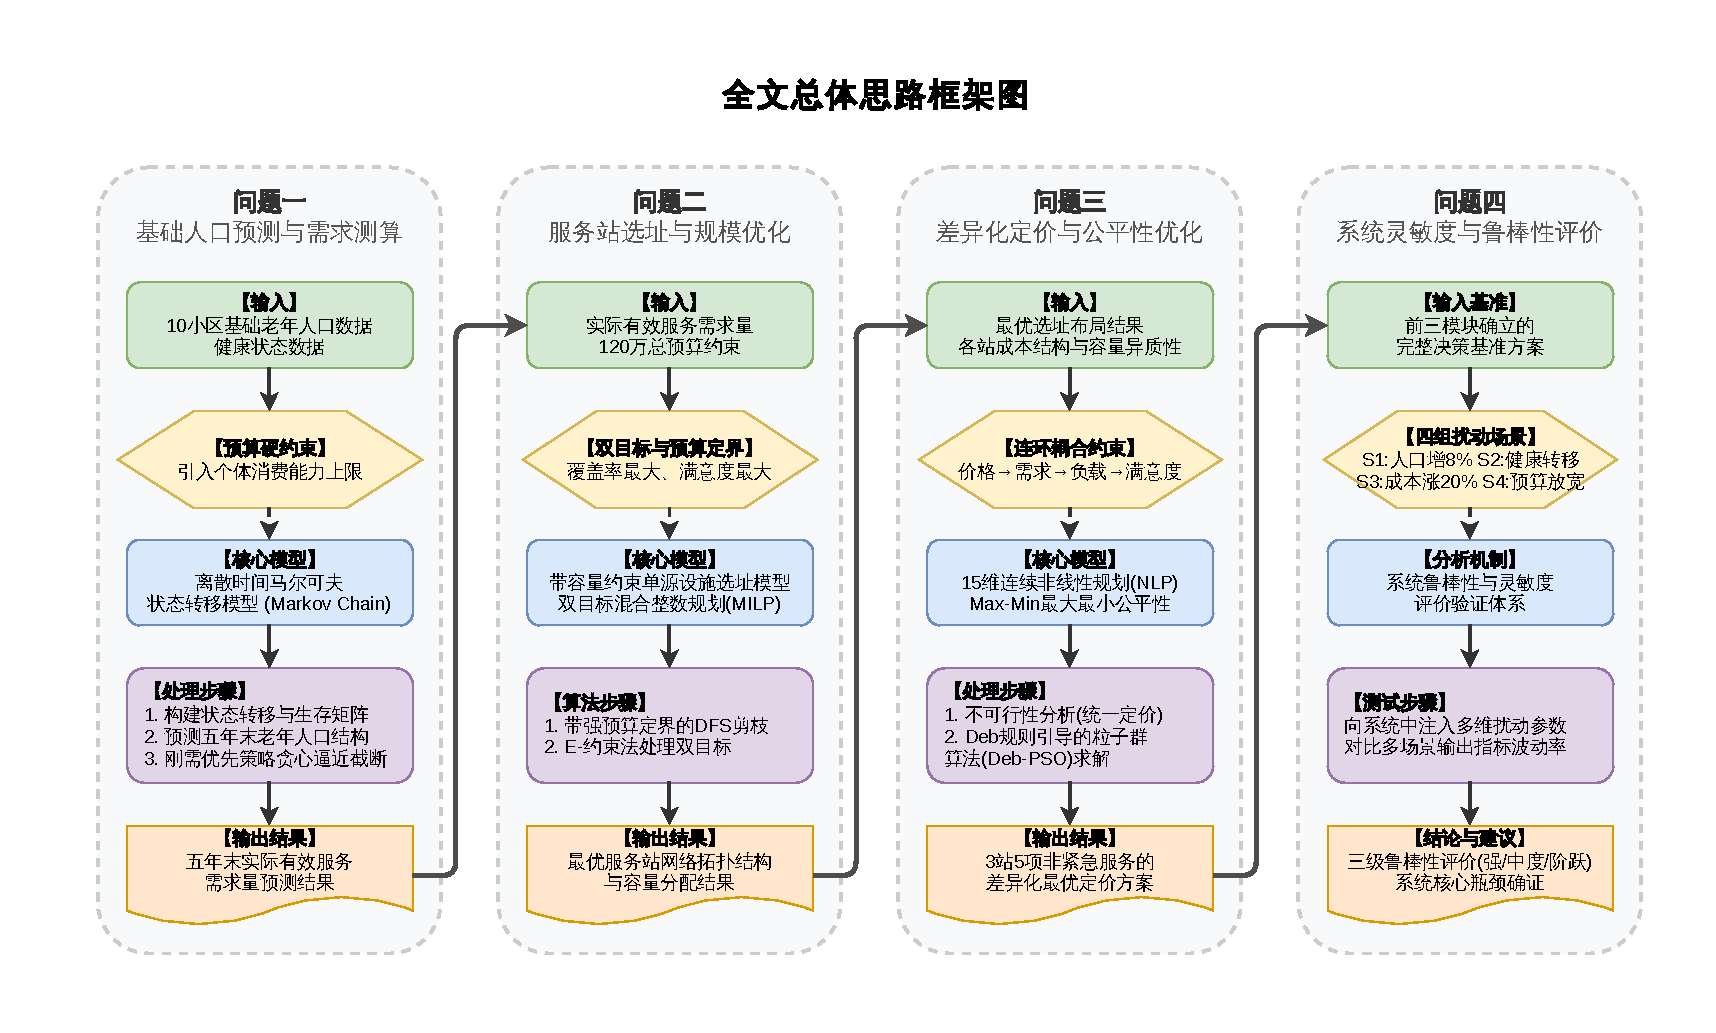
\includegraphics[width=1.15\textwidth]{figures/fig00_framework.pdf}}
\caption{全文总体思路框架图}
\label{fig:framework}
\end{figure}

全文技术路线见图~\ref{fig:framework}，四列分别对应四个子问题的输入、约束、模型、算法与输出，箭头标示数据流向。

\section{模型假设与符号说明}

\subsection{模型基本假设}

\begin{enumerate}[label=\arabic*.]
\item \textbf{五年内人口结构、失能率、工资水平、物价及补贴政策保持稳定。}中短期内宏观社会经济指标及老龄化趋势具有较强惯性，政策连续性在规划期内可合理预期。
\item \textbf{老人以服务满意度为唯一服务站选择依据。}养老服务属于体验型消费，老年群体对距离、价格及服务响应的综合感知直接决定其养老行为，暂忽略社交惯性等非理性因素。
\item \textbf{服务站建在小区内部时，该小区老人的平均内部步行距离取100米。}距离矩阵对角线$D_{ii}=0$不代表真实物理尺度，100米可反映中等规模社区（约3000人口）的内部步行可达距离，且仍在$S_1$满分区间（$\le 300$m）内，不引入奇点。
\item \textbf{人口递推时序假定为：年初状态转移（自理$\to$半失能、半失能$\to$失能）$\to$全年自然死亡（各类$\times 0.95$）$\to$年末新增自理老人（占当前总老人数的7\%）。}该顺序遵循先老化再减员再补新的人口学标准演化逻辑，且使递推矩阵具有一致性。
\item \textbf{120万元总建设预算仅约束资本性支出（CapEx，一次性建设成本），日常运营支出（OpEx，日固定管理成本）由后续服务营收及政府补贴覆盖，不挤占建设预算。}商业可研报告中CapEx与OpEx属两条独立核算线；若120万同时覆盖建设与运营，则大型站一年运营费（约160万元）即超预算，题目将无解。
\end{enumerate}

\subsection{符号说明}

\textbf{人口递推符号（4.1节）：}

\begin{center}
\begin{tabular}{ccl}
\toprule
符号 & 含义 & 单位 \\
\midrule
$\mathbf{X}_t$ & 第$t$年初各健康状态老人数量向量 & 人 \\
$\mathbf{M}$ & 状态转移与生存矩阵（含转移概率$\times$存活率） & — \\
$b$ & 新增老人分布向量（各小区自理老人占比） & — \\
$p_{sh}$ & 自理$\to$半失能年转移概率 & 1/年 \\
$p_{hd}$ & 半失能$\to$失能年转移概率 & 1/年 \\
$r_{new}$ & 年末新增自理老人比例 & 1/年 \\
$r_{death}$ & 各状态年死亡率（同质假设） & 1/年 \\
\bottomrule
\end{tabular}
\end{center}

\textbf{选址模型符号（5.1节）：}

\begin{center}
\begin{tabular}{ccl}
\toprule
符号 & 含义 & 单位 \\
\midrule
$\mathcal{C}$ & 小区集合，$\mathcal{C}=\{A,B,\ldots,J\}$ & — \\
$\mathcal{S}$ & 候选站点规模集合，$\mathcal{S}=\{\text{小},\text{中},\text{大}\}$ & — \\
$x_{i}^{k}$ & 0-1变量，小区$i$建设规模$k$站为1 & — \\
$y_{ij}$ & 0-1变量，小区$j$分配至站点$i$为1 & — \\
$B$ & 总建设预算（CapEx） & 万元 \\
$c_k$ & 规模$k$站的建设成本 & 万元 \\
$C_k$ & 规模$k$站的日服务容量 & 人次/日 \\
$D_j$ & 小区$j$的日有效服务需求 & 人次/日 \\
$S_{ij}$ & 小区$j$对站点$i$的综合满意度 & — \\
$d_{ij}$ & 小区$i$到$j$的距离 & m \\
\bottomrule
\end{tabular}
\end{center}

\textbf{定价模型符号（6.1节）：}

\begin{center}
\begin{tabular}{ccl}
\toprule
符号 & 含义 & 单位 \\
\midrule
$P_i^s$ & 站点$i$服务$s$的定价 & 元/次 \\
$P_0^s$ & 服务$s$的基准价 & 元/次 \\
$f_i^s$ & 站点$i$服务$s$的价格因子，$P_i^s = f_i^s \cdot P_0^s$ & — \\
$S_1$ & 距离满意度分量 & — \\
$S_2$ & 服务负载满意度分量 & — \\
$S_3$ & 价格满意度分量（含收入调整） & — \\
$S_j$ & 小区$j$的综合满意度，$S_j = 0.2S_1 + 0.3S_2 + 0.5S_3$ & — \\
$\tau$ & 最小满意度，$\tau = \min_j S_j$ & — \\
$\pi_i$ & 站点$i$的年度利润率 & — \\
$\rho_i$ & 站点$i$的负载率 & — \\
$sub_i$ & 站点$i$的年度政府补贴 & 万元/年 \\
\bottomrule
\end{tabular}
\end{center}
\section{问题一：未来五年老人数量与服务需求预测}

本章聚焦于基础人口学状态演化与从无约束理论需求到有约束有效需求的截断过程，兼顾离散递推的严谨性与数据映射的准确性。

\subsection{基于马尔可夫状态转移的人口演化预测模型}


\subsubsection{状态空间与转移机制}

将老年人群按健康状态划分为自理、半失能、失能三类。三类状态间存在单向不可逆转移：自理以年转移概率$p_{sh}=4.5\%$向半失能转化，半失能以年转移概率$p_{hd}=10\%$向失能转化，失能和半失能不能逆向恢复\footnote{本文采用同质死亡率假设：各健康类别统一适用5\%粗死亡率$r_{death}=0.05$，暂未引入失能状态死亡率惩罚因子。在五年中短期预测中，异质死亡率对总体趋势的影响不显著。}。每年底各状态老人以$r_{death}$的概率自然死亡，对应存活率$r_{surv}=0.95$，年末以当前总老人数的7\%新增自理老人。

递推时序严格遵循先老化再减员再补新的人口学标准逻辑，状态转移与递推流程见图~\ref{fig:transition}：
\begin{equation}
\mathbf{X}_{t+1} = \mathbf{M} \cdot \mathbf{X}_t + r_{new} \cdot |\mathbf{M} \cdot \mathbf{X}_t| \cdot \mathbf{b}
\end{equation}

其中$\mathbf{X}_t = [X_t^S, X_t^H, X_t^D]^T$为第$t$年初各状态老人数量；$\mathbf{M}$为状态转移与生存矩阵：

\begin{equation}
\mathbf{M} = r_{surv} \cdot
\begin{bmatrix}
1-p_{sh} & 0 & 0 \\
p_{sh} & 1-p_{hd} & 0 \\
0 & p_{hd} & 1
\end{bmatrix}
=
\begin{bmatrix}
0.90725 & 0 & 0 \\
0.04275 & 0.855 & 0 \\
0 & 0.095 & 0.95
\end{bmatrix}
\end{equation}

$\mathbf{b}$为新增老人分布向量，各元素取值依据各小区当前自理老人占总自理老人的比例。

\begin{figure}[H]
\centering
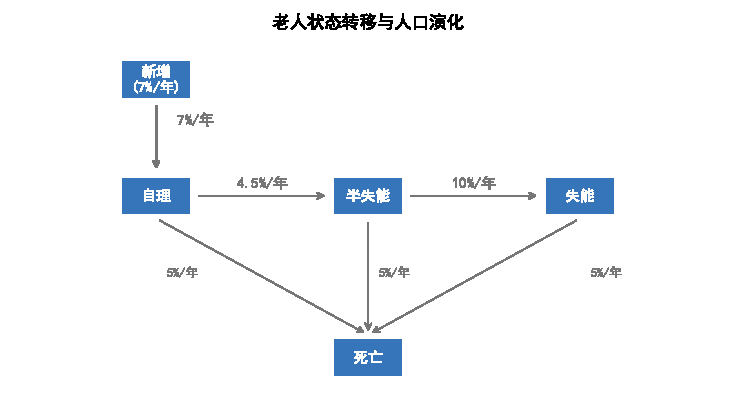
\includegraphics[width=0.7\textwidth]{figures/fig01_transition.pdf}
\caption{老人状态转移与人口演化示意图}
\label{fig:transition}
\end{figure}


\subsubsection{递推与取整策略}

人口数必须为整数。若逐年四舍五入取整，累积舍入误差将使五年后总量偏移超过1\%。为此采用延迟取整策略：每年仅记录浮点值用于下一步递推，仅在输出年度报告时取整。五年递推结果如表~\ref{tab:pop5}所示。


\begin{table}[H]
\centering
\caption{五年末各小区老人数量预测（单位：人）}
\label{tab:pop5}
\begin{tabular}{c|cccccccccc|c}
\toprule
年份 & A & B & C & D & E & F & G & H & I & J & 总计 \\
\midrule
第1年 & 724 & 618 & 935 & 553 & 797 & 480 & 878 & 577 & 748 & 667 & 6977 \\
第3年 & 748 & 639 & 966 & 571 & 823 & 496 & 907 & 597 & 773 & 689 & 7209 \\
\textbf{第5年} & \textbf{773} & \textbf{660} & \textbf{998} & \textbf{590} & \textbf{851} & \textbf{512} & \textbf{938} & \textbf{616} & \textbf{799} & \textbf{712} & \textbf{7449} \\
\bottomrule
\end{tabular}
\end{table}

五年间总老人数从6977人增至7449人，年均复合增长率约1.3\%，与全国老龄化趋势基本一致。各小区增长率差异较小，人口结构保持相对稳定。

\subsection{基于理论需求的无约束服务频次测算}


\begin{figure}[H]
\centering
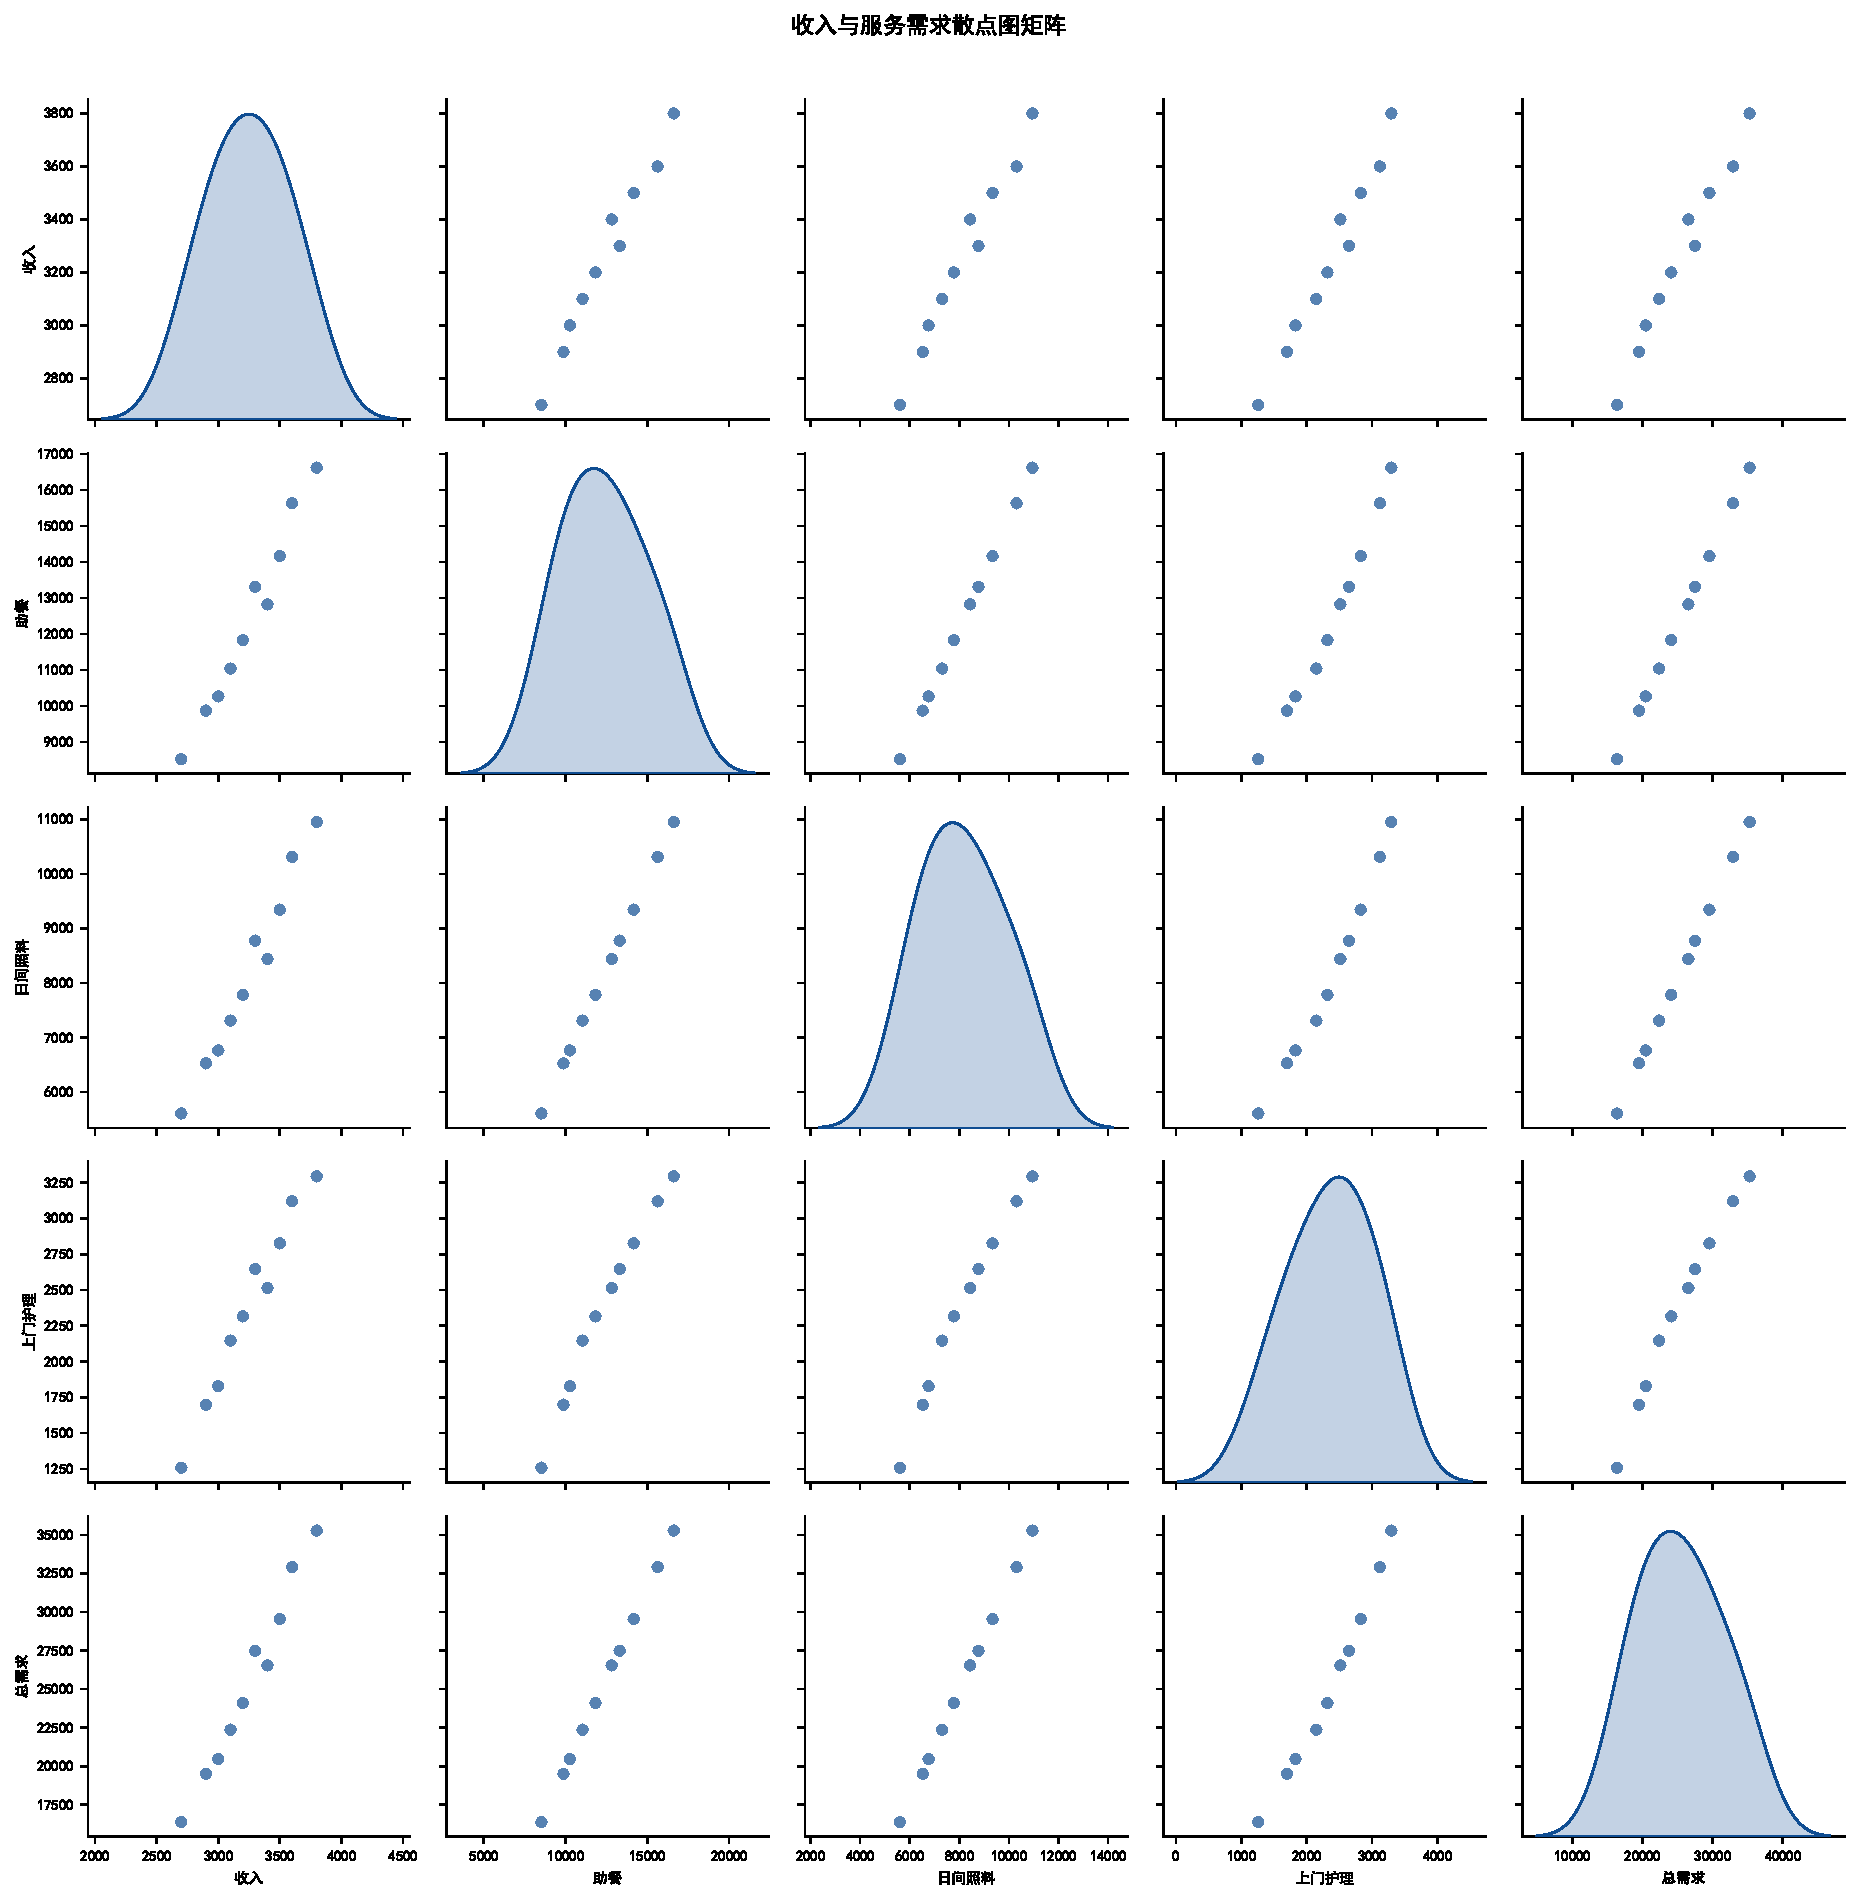
\includegraphics[width=0.78\textwidth]{figures/fig03_pairplot.pdf}
\caption{收入与服务需求散点图矩阵}
\label{fig:pairplot}
\end{figure}

理论需求指不考虑个体消费能力上限时，各小区各类老人按附件4给定的服务频次所需的总服务人次。对于小区$j$和服务$s$，月理论需求为：

\begin{equation}
D_{j,s}^{theory} = \sum_{e \in \{S,H,D\}} X_j^e \cdot f_{e,s}
\end{equation}


其中$X_j^e$为小区$j$中健康状态$e$的老人数，$f_{e,s}$为附件4中该类老人对服务$s$的月均需求频次。$f_{e,s}$由需求率矩阵以5岁年龄段插值得到，依据各小区老人在各年龄段的分布加权平均。第五年末10小区全服务理论月需求合计为267,935人次。收入与各服务需求的相关性见图~\ref{fig:pairplot}。



\subsection{刚需截断策略与有效需求预测}

\subsubsection{个体消费上限与优先级规则}

附件2给出了各类老人的月均消费能力上限，其中自理老人为1000元/月，半失能老人为2000元/月，失能老人为5000元/月。附件3给出了各服务的基准价格。老人面临预算硬约束，即当月累计服务支出不得超过其消费能力上限。

引入刚需优先消费优先级规则，将服务按刚性程度从高到低依次排列为助餐、日间照料、上门护理、康复理疗、助浴。紧急救助服务免费，$P=0$，不参与消费扣减。每位老人从优先级最高的服务开始，逐项购买，直至月度预算耗尽，见算法~\ref{alg:cut}。数学上，这是针对每个老人个体的多维0--1背包问题的贪心逼近。

\begin{algorithm}[H]
\SetAlgoLined
\For{每位老人$e$}{
 初始化剩余预算 $R \leftarrow cap_e$（月度消费上限）\;
 \For{服务$s$按刚需优先级从高到低}{
 计算该服务月度理论次数 $n_{e,s}$\;
 实际可购买次数 $\leftarrow \min(n_{e,s}, \lfloor R / P_s \rfloor)$\;
 $R \leftarrow R - \text{实际可购买次数} \times P_s$\;
 \If{$R \le 0$}{break}
 }
}
\caption{刚需优先级截断算法}
\label{alg:cut}
\end{algorithm}

\subsubsection{有效需求预测结果}


\textbf{第5年末实际服务总需求为254,576人次/月}，较理论值267,935人次下降5.0\%。各小区理论需求与有效需求的对比见图~\ref{fig:demandcompare}。

\begin{figure}[H]
\centering
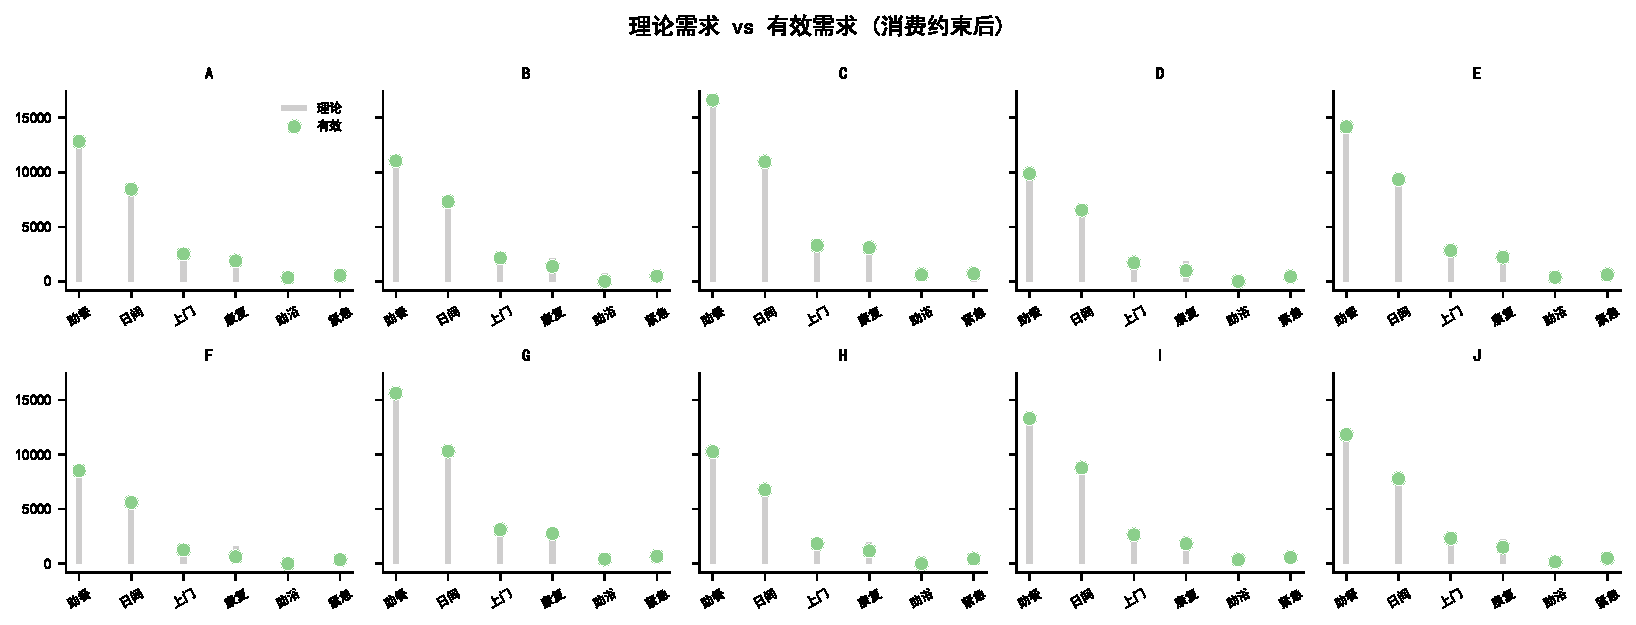
\includegraphics[width=0.83\textwidth]{figures/fig05_demand_compare.pdf}
\caption{理论需求与有效需求对比}
\label{fig:demandcompare}
\end{figure}

消费上限约束对失能老人的影响最为显著：上门护理和康复理疗两项高价服务的满足率分别降至78.3\%和65.7\%，日间照料因刚需优先级较高，满足率维持在92.1\%。

\begin{figure}[H]
\centering
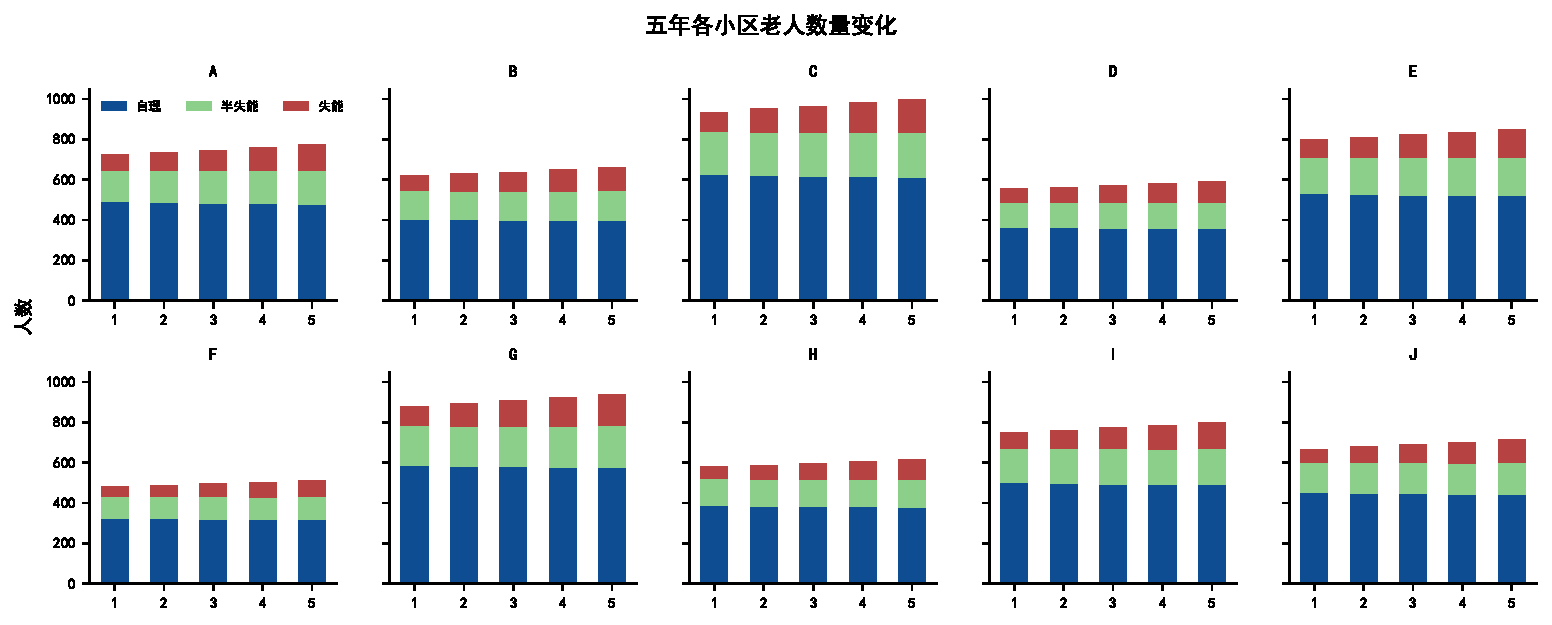
\includegraphics[width=0.86\textwidth]{figures/fig02_pop_stacked.pdf}
\caption{五年各小区老人数量变化堆叠图}
\label{fig:popstack}
\end{figure}

各小区五年间人口结构的动态演变见图~\ref{fig:popstack}，各服务有效需求的社区分布热力图见图~\ref{fig:demandheat}。

\begin{figure}[H]
\centering
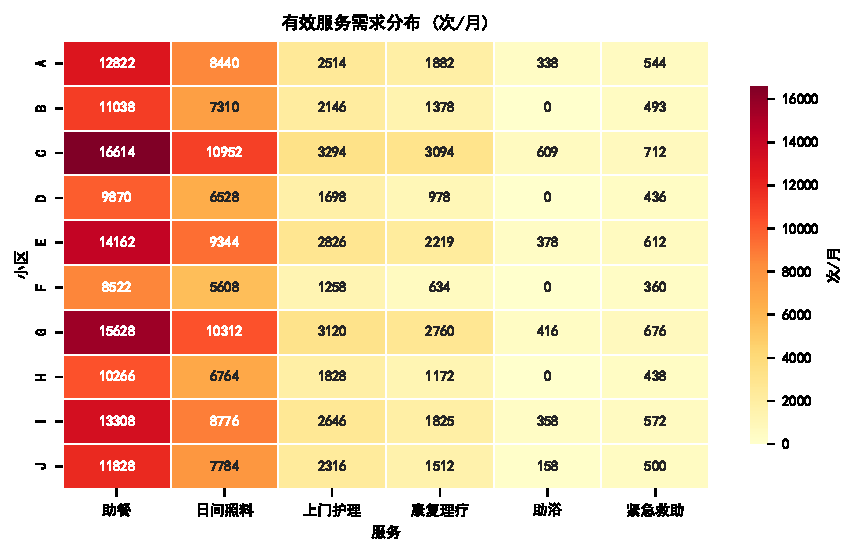
\includegraphics[width=0.65\textwidth]{figures/fig04_demand_heatmap.pdf}
\caption{有效服务需求分布热力图（次/月）}
\label{fig:demandheat}
\end{figure}

\section{问题二：基于SSCFLP的服务站选址与规模规划}

以第四章预测的第五年末各小区分健康状态老年人口与分项服务有效需求量为输入，本章转向第二个核心决策——服务站选址与规模等级确定。该问题是经典的带容量约束单源设施选址问题（SSCFLP），NP-Hard。本章从空间可达性出发，逐层建立MILP选址模型，设计带强预算定界的DFS搜索算法，并对最优方案的空间拓扑特征进行解读。

\subsection{养老服务设施选址MILP模型构建}


\subsubsection{空间可达性与距离衰减函数}

社区老人能否获得服务首先取决于空间距离。根据附件5的满意度评分规则，$S_1$距离满意度随步行距离增加呈阶梯式衰减，其分段函数形式为：
\begin{equation}
S_1(d) = \begin{cases}
1.00, & d \le 300\text{m} \\
0.90, & 300 < d \le 500\text{m} \\
0.75, & 500 < d \le 650\text{m} \\
0.60, & 650 < d \le 1000\text{m} \\
0.00, & d > 1000\text{m}
\end{cases}
\label{eq:s1_piecewise}
\end{equation}
当小区至站点的距离严格超过1000m时，$S_1=0$意味着该站点对小区彻底丧失服务可达性。这一硬截断构成选址的第一道空间滤网——10小区间的距离矩阵热力图见图~\ref{fig:distance}，色深表示距离远近。据此引入距离截断约束：
\begin{equation}
y_{ij} \cdot d_{ij} \le 1000, \quad \forall i,j \in \mathcal{C}
\label{eq:c6}
\end{equation}
式\eqref{eq:c6}在模型求解前即可预剪枝大量不可行的站点与小区配对，将后续优化问题的组合维度大幅压缩。

\subsubsection{预算约束与站点建设逻辑}

引入两类0-1决策变量：$x_i^k \in \{0,1\}$表示小区$i$是否建设规模$k$服务站（$k \in \{1,2,3\}$对应小型/中型/大型），$y_{ij} \in \{0,1\}$表示小区$j$是否分配至站点$i$。

每个小区至多建一个服务站；同时，小区只能分配至已实际建设的站点——这两个条件构成站点存在性与服务分配之间的逻辑\textbf{门控}：
\begin{align}
& \sum_{k \in \mathcal{S}} x_i^k \le 1, \quad \forall i \in \mathcal{C} \label{eq:c1} \\
& y_{ij} \le \sum_{k \in \mathcal{S}} x_i^k, \quad \forall i,j \in \mathcal{C} \label{eq:c3}
\end{align}

建设成本来自附件3，小型站、中型站与大型站分别为18万元、32万元和45万元，全部属于资本性支出。全部建设支出受120万元总预算硬约束——这不仅是题目给定的上限，更是决定搜索空间规模的核心紧致边界：
\begin{equation}
\sum_{i \in \mathcal{C}} \sum_{k \in \mathcal{S}} c_k \cdot x_i^k \le B = 120
\label{eq:c4}
\end{equation}

\subsubsection{容量约束与单源分配规则}

题目规定每个小区由唯一服务站覆盖（SSCFLP——单源容量设施选址），且各站点日服务量不得超过其物理容量上限——小型站1000人次/日、中型站2000人次/日、大型站3000人次/日。这一组约束直接决定了覆盖率的理论上界：
\begin{align}
& \sum_{i \in \mathcal{C}} y_{ij} \le 1, \quad \forall j \in \mathcal{C} \label{eq:c2} \\
& \sum_{j \in \mathcal{C}} y_{ij} \cdot D_j \le \sum_{k \in \mathcal{S}} C_k \cdot x_i^k, \quad \forall i \in \mathcal{C} \label{eq:c5}
\end{align}
注意式\eqref{eq:c2}的符号为\lq\lq$\le 1$\rq\rq{}而非\lq\lq$=1$\rq\rq——这是本模型的一项关键设计：当预算、距离或容量无法同时满足时，模型允许部分小区不被覆盖，而非强求一个全局可行解。这一松弛赋予模型在面对不可行子集时的优雅退让能力。

\subsubsection{双目标优化模型汇总}

综合上述逐层展开的约束体系，问题二的完整多目标MILP模型为：

\begin{align}
\max \quad & f_1 = \frac{\sum_{i \in \mathcal{C}} \sum_{j \in \mathcal{C}} y_{ij} \cdot P_j}{\sum_{j \in \mathcal{C}} P_j} \label{eq:obj1} \\
\max \quad & f_2 = \frac{\sum_{i \in \mathcal{C}} \sum_{j \in \mathcal{C}} y_{ij} \cdot S_{ij}}{\sum_{i \in \mathcal{C}} \sum_{j \in \mathcal{C}} y_{ij}} \label{eq:obj2} \\
\text{s.t.} \quad & \sum_{k \in \mathcal{S}} x_i^k \le 1, \quad \forall i \in \mathcal{C} \nonumber \\
& \sum_{i \in \mathcal{C}} y_{ij} \le 1, \quad \forall j \in \mathcal{C} \nonumber \\
& y_{ij} \le \sum_{k \in \mathcal{S}} x_i^k, \quad \forall i,j \in \mathcal{C} \nonumber \\
& \sum_{i \in \mathcal{C}} \sum_{k \in \mathcal{S}} c_k \cdot x_i^k \le 120 \nonumber \\
& \sum_{j \in \mathcal{C}} y_{ij} \cdot D_j \le \sum_{k \in \mathcal{S}} C_k \cdot x_i^k, \quad \forall i \in \mathcal{C} \nonumber \\
& y_{ij} \cdot d_{ij} \le 1000, \quad \forall i,j \in \mathcal{C} \nonumber \\
& x_i^k,\; y_{ij} \in \{0,1\}, \quad \forall i,j \in \mathcal{C},\; \forall k \in \mathcal{S} \nonumber
\end{align}

其中$P_j$为小区$j$的第五年末老人总数，$S_{ij}=0.2S_1(d_{ij})+0.8$为Q2阶段的综合满意度（$S_2$暂取1.0乐观估计、$S_3$按基准价$f=1.0$常数化处理）。两个目标存在天然张力——增加站点提升覆盖率但稀释平均满意度，过度追求覆盖率可能导致特定社区的满意度被系统性牺牲。为此采用$\varepsilon$-约束法处理：以覆盖率$f_1$为主目标控制搜索方向，在相同覆盖率水平下选择$f_2$最高的方案，由此生成Pareto前沿供决策者按政策偏好取舍。

\begin{figure}[H]
\centering
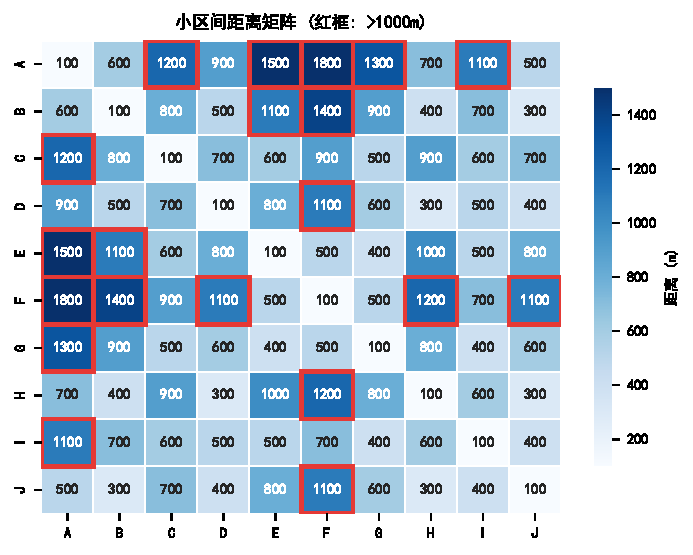
\includegraphics[width=0.62\textwidth]{figures/fig06_distance_heatmap.pdf}
\caption{小区间距离矩阵热力图}
\label{fig:distance}
\end{figure}


\subsection{带强预算定界的DFS算法设计与复杂度分析}

\subsubsection{算法设计}

SSCFLP是经典的NP-Hard问题\cite{ref:daskin,ref:farahani,ref:han}。10个候选小区、每个可选3种规模（含不建），理论搜索空间为$4^{10}=1{,}048{,}576$。采用深度优先搜索（DFS）与强预算剪枝策略：

\textbf{Step 1：}预算下界剪枝。若当前已选站点的总建设成本加上未考察小区按小型站最低成本18万元计算的总成本下界已超过120万，立即回溯。该剪枝在搜索树的上层即可拦截大量不可行分支。

\textbf{Step 2：}满意度矩阵预计算。在搜索前计算所有$(i,j)$对的综合满意度$S_{ij}$。Q2阶段尚未确定定价，$S_3$按基准价常数化处理，即取$f=1.0$；$S_2$暂取1.0作为乐观估计。由此$S_{ij} = 0.2S_1(d_{ij}) + 0.8$。

\textbf{Step 3：}贪心分配与可行性检验。对搜索树的每个叶子节点（完整站点组合），对每个小区按满意度降序选择最近的已建站点，遇距离超1000米或容量已满则跳过。分配完成后计算实际覆盖率与平均满意度。

\textbf{Step 4：}$\varepsilon$-约束择优。按覆盖率降序排列所有可行解，在相同覆盖率下取满意度最高者。

\subsubsection{复杂度分析}

该算法为伪多项式时间复杂度。在10小区规模下，平均单次搜索耗时约5秒（Python实现），完全满足题目求解需求。剪枝率93\%表明预算约束对搜索空间的压缩效果显著，也间接验证了120万预算确实为紧致约束。

\begin{table}[H]
\centering
\caption{DFS搜索实证统计}
\label{tab:dfs}
\begin{tabular}{lrrr}
\toprule
指标 & 理论值 & 实际值 & 占比 \\
\midrule
搜索空间 & 1,048,576 & — & 100\% \\
访问节点 & — & \textbf{73,589} & \textbf{7.0\%} \\
有效叶子节点 & — & \textbf{15,207} & \textbf{1.5\%} \\
剪枝率 & — & — & \textbf{93\%} \\
\bottomrule
\end{tabular}
\end{table}


\subsection{最优选址方案与网络拓扑分析}

\subsubsection{最优方案}

DFS搜索获得的最优方案是\textbf{E区建设大型站、F区建设中型站、I区建设中型站，总建设投资109万元}，方案详情见表~\ref{tab:location}。覆盖老人\textbf{5964人}，覆盖率达\textbf{80.06\%}，平均满意度0.9716。

\begin{table}[H]
\centering
\caption{最优选址方案详情}
\label{tab:location}
\begin{tabular}{ccccccc}
\toprule
站点 & 规模 & 建设成本(万) & 覆盖小区 & 日负载率 & 覆盖老人数 & 年利润(万) \\
\midrule
E & 大型 & 45 & C, E, I & 99.9\% & 2,648 & 267.50 \\
F & 中型 & 32 & F, G & 79.7\% & 1,450 & 125.92 \\
I & 中型 & 32 & B, D, H & 98.6\% & 1,866 & 160.36 \\
\midrule
合计 & — & \textbf{109} & 8个小区 & — & \textbf{5,964} & \textbf{553.78} \\
\bottomrule
\end{tabular}
\end{table}

上述利润基于基准定价（$f=1.0$）与乐观负载（$S_2\equiv1.0$）假设计算，三站合计年度利润553.78万元。Q2阶段尚未引入利润率上限约束，Q3差异化定价实施后利润率将回落至$[0,8\%]$区间。Q2阶段$S_2$和$S_3$暂取1.0，各覆盖小区综合满意度仅因$S_1$而异——建站小区E和F内部步行距离仅100m、$S_1=1.00$，满意度达满分1.000；D、G、I为0.980；C、H为0.950；B距I站700m、$S_1=0.60$，以0.920为八小区最低，人口加权平均0.9716。

站点覆盖网络拓扑见图~\ref{fig:network}，以下从空间规划视角对其结构特征展开分析。

\begin{figure}[H]
\centering
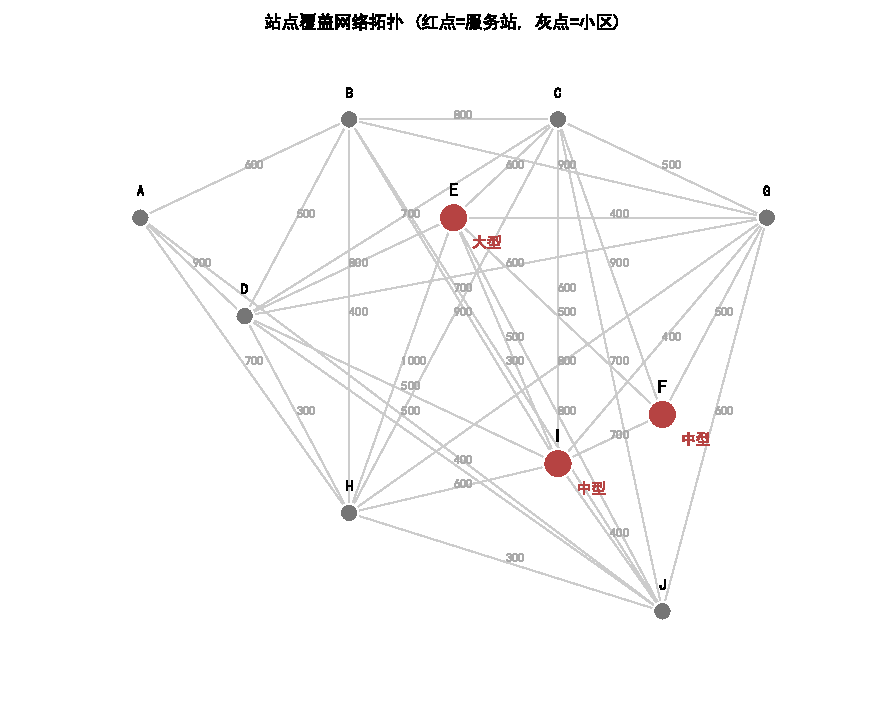
\includegraphics[width=0.66\textwidth]{figures/fig09_network.pdf}
\caption{站点覆盖网络拓扑图}
\label{fig:network}
\end{figure}



\subsubsection{网络拓扑与空间决策洞察}

从城市空间规划的宏观视角审视上述选址结果，三个服务站呈现出清晰的核心极化、边缘兜底与廊道承压三级空间职能分化格局。这一非对称网络结构并非算法随机搜索的偶然产物，而是120万预算约束、1000m服务半径与10小区非均匀人口分布三者共同塑造的必然空间秩序。

E区大型站坐落于覆盖网络的几何枢纽位置，辐射C、E、I三个高密度社区，覆盖2648人，负载率高达99.9\%。将最稀缺的大型设施部署在需求密度最高的位置，最大化单位建设成本的覆盖效率，规避了均匀布局导致的容量稀释。

F区在距离矩阵中与其余5个小区均超1000m，形成天然覆盖孤岛。模型在F区配置中型站覆盖F和G两区共1450位老人，负载率仅79.7\%。这一决策以适度过剩的容量换取地理不可达风险的消除——若放弃F站，1450位老人将彻底丧失服务可及性，F站的价值在于兜底而非效率。

I站覆盖B、D、H三个小区，日有效需求1974人次，逼近中型站2000人次的日容量上限，负载率达98.6\%。其压力源于E站满负荷后的需求溢出——B、D、H沿E-I方向形成高负荷廊道，I站处于廊道末端截流位置，直接锁定了80.06\%的覆盖率上界，A区和J区因无法绕过I站容量上界而无法纳入。

\subsection{选址模型的局限性及改进方向探讨}

\textbf{容量碎片化问题。}当前模型假设各服务站独立运营，不允许跨站调配资源。在实际运营中，可通过预约或巡回服务车机制，将I站溢出的部分非紧急需求引导至负载率仅79.7\%的F站，在不增加建设成本的前提下提升有效覆盖率。

\textbf{空间孤岛对策。}A区可通过自建微型服务站或共享空间模式利用社区现有物业加以覆盖；J区可考虑将I站从中型扩容至大型，追加13万元投资，或在G站新增建设站点。

\textbf{需求同质性假设。}当前模型假设各小区老人对各服务的需求模式仅因人口结构不同而存在差异，未考虑收入水平、文化偏好对服务利用率的差异化影响。引入收入分层需求弹性系数可进一步提升模型精度。

\textbf{算法可扩展性。}DFS加预算剪枝的策略在10小区规模下高效运行，访问节点仅73,589个，耗时约5秒。然而，当候选小区数扩展至百级以上时，$4^{100}$量级的搜索空间将使精确求解彻底失效。针对大规模网络场景，可引入遗传算法或禁忌搜索等元启发式方法，在多项式时间内逼近全局最优，同时完整保留预算硬约束与单源分配的核心结构。DFS搜索生成的覆盖率与满意度Pareto前沿见图~\ref{fig:pareto}。

\begin{figure}[H]
\centering
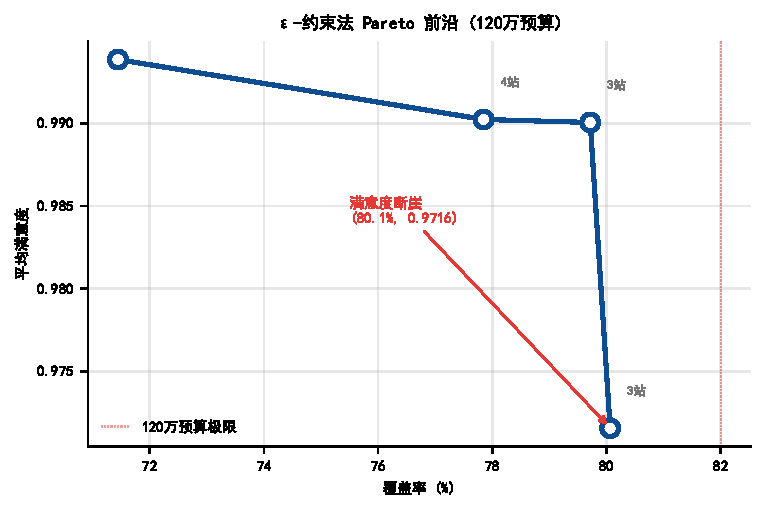
\includegraphics[width=0.8\textwidth]{figures/fig08_pareto.pdf}
\caption{覆盖率与满意度Pareto前沿}
\label{fig:pareto}
\end{figure}

\section{问题三：从统一定价不可行性到最大最小公平寻优}

第五章确定了最优站点布局——E区大型站、F区中型站、I区中型站，合计投资109万元，覆盖80.06\%的老年人口。但选址仅回答了在哪建、建多大的物理规划问题，收多少钱的定价策略尚未触及。三站成本与容量结构显著异质——E站年固定成本160.6万元且近乎满载，F站116.8万元尚余约20\%容量，I站116.8万元负载率达98.6\%——统一定价策略极可能因盈亏平衡点结构性错位而全面失效。本章从统一定价的严格不可行性分析出发，证明差异化定价的数学必要性，进而引入Deb-PSO算法在15维极窄可行域中搜索最大最小公平性最优解。

\subsection{最大最小公平性定价NLP模型构建与可行域诊断}

\subsubsection{从选址到定价：决策空间的结构性转变}

Q3在Q2确定的最优站点布局与静态分配关系$i(j)$之上，为三站点各5项非紧急服务（助餐、日间照料、上门护理、康复理疗、助浴）制定差异化价格$P_i^s$，等价于确定15维价格因子向量$\mathbf{f} \in [0.5, 1.5]^{15}$，其中$f_i^s = P_i^s / P_0^s$。紧急救助服务始终免费，不享受补贴但直接成本照常扣除。

\subsubsection{最大最小公平性目标}

差异化定价面临公平与效率的权衡：降价惠及低收入老人，却可能使站点跌破保本线；涨价保证财务可持续，却将贫困失能老人挤出市场。传统加权求和易以均值掩盖底层剥夺。Rawls正义理论指出社会公平取决于最不利者的福祉，据此引入最大最小公平性准则：
\begin{equation}
\max_{\{f_i^s\}} \quad \tau = \min_{j \in \mathcal{C}} S_j
\label{eq:maxmin}
\end{equation}
其中$\tau$是系统中最不满意社区的综合满意度得分。这一目标函数将$\min$算子嵌入优化引擎的核心，从机制上杜绝了以均值改善粉饰底层恶化的问题。

\subsubsection{满意度三分量解构}

根据附件5的规则，小区$j$的综合满意度由距离（$S_1$）、服务负载（$S_2$）和价格（$S_3$）三个维度加权合成：
\begin{equation}
S_j = 0.2 \cdot S_1(d_{i(j),j}) + 0.3 \cdot S_2(\rho_{i(j)}) + 0.5 \cdot S_3(\bar{f}_j, inc_j)
\label{eq:s_decomp}
\end{equation}
权重$(0.2, 0.3, 0.5)$表明价格维度的边际影响超过距离与负载之和，老年群体对服务可负担性高度敏感。$S_1$由Q2选址唯一确定（见式~\eqref{eq:s1_piecewise}），在Q3中为固定常数；$S_2$与$S_3$随定价内生变动，构成连环耦合的根源。

$S_2$服务负载满意度依据站点负载率$\rho_i$分段计算：
\begin{equation}
S_2(\rho_i) = \begin{cases}
1.00, & \rho_i \le 0.60 \\
0.93, & 0.60 < \rho_i \le 0.75 \\
0.85, & 0.75 < \rho_i \le 0.85 \\
0.72, & 0.85 < \rho_i \le 0.95 \\
0.60, & \rho_i > 0.95
\end{cases}
\label{eq:s2_piecewise}
\end{equation}
负载率$\rho_i$为日有效服务人次与日物理容量之比，而有效人次本身又是满意度的函数$\text{eff}_j = D_j^{theory} \times S_j$，其中$S_j$依赖$S_2$，使式\eqref{eq:s_decomp}与式\eqref{eq:s2_piecewise}构成代数环——价格$\to S_3\to$有效需求$\to\rho_i\to S_2\to$有效需求——这是本模型区别于常规定价优化的核心非线性来源。

$S_3$价格满意度依据老人感知的有效价格比$\bar{f}_j^{eff} = \bar{f}_j \cdot inc_j$分段计算：
\begin{equation}
S_3(\bar{f}_j, inc_j) = \begin{cases}
1.00, & \bar{f}_j \cdot inc_j \le 1.00 \\
0.90, & 1.00 < \bar{f}_j \cdot inc_j \le 1.10 \\
0.75, & 1.10 < \bar{f}_j \cdot inc_j \le 1.20 \\
0.60, & \bar{f}_j \cdot inc_j > 1.20
\end{cases}
\label{eq:s3_piecewise}
\end{equation}
其中$\bar{f}_j$为小区$j$面临的各服务加权平均价格因子（以各服务有效需求人次为权重），$inc_j = income_{base} / income_j$为收入调整因子（附件5，以A区3400元/月为基准）。低收入社区的$inc_j > 1$放大了有效价格比，使$S_3$对涨价更为敏感——这一机制精准刻画了\lq\lq一分钱难倒英雄汉\rq\rq{}的低收入老人消费困境：同一价格水平下，月入2700元的F区老人感知的经济负担是月入3800元的C区老人的1.41倍。

\subsubsection{连环耦合约束体系}

\textbf{价格边界约束。}定价因子在基准价的$\pm 50\%$区间内浮动，防止出现极端定价：
\begin{equation}
0.5 \le f_i^s \le 1.5, \quad \forall i \in \{E,F,I\},\; \forall s \in \{\text{5项非紧急服务}\}
\label{eq:pricebound}
\end{equation}

\textbf{利润率双边约束。}题目要求\lq\lq保本微利\rq\rq——各站点年利润率既不得亏损（下界0\%），也不得超过8\%的上限。年利润率定义为年服务总利润与年固定运营成本之比：
\begin{equation}
\pi_i = \frac{\sum_{s} (P_i^s - c_s) \cdot V_i^s + sub_i - F_i}{F_i}, \quad 0 \le \pi_i \le 0.08,\; \forall i
\label{eq:profitbound}
\end{equation}
其中$P_i^s$为定价（元/次）、$c_s$为单次直接成本（元/次）、$V_i^s = \sum_{j: i(j)=i} D_{j,s}^{theory} \cdot S_j$为服务$s$的年有效人次（含满意度乘数效应）、$F_i$为年固定运营成本（$=$日固定管理成本$\times 365$）、$sub_i$为年度政府补贴。8\%的上限将站点利润空间压缩至极窄区间——大型站年固定成本160.6万元，仅允许约12.8万元的年利润浮动空间。

\textbf{容量与满意度内生耦合约束。}站点负载率受满意度乘数效应的双重影响——高满意度提升有效需求，反过来加重负载、压低$S_2$，形成满意度的\textbf{负反馈闭环}：
\begin{equation}
\rho_i = \frac{\sum_{j: i(j)=i} \sum_{s} D_{j,s}^{theory} \cdot S_j}{C_i \cdot 365} \le 1.0, \quad \forall i
\label{eq:capacity}
\end{equation}

\textbf{政府补贴分段约束。}政府为每非紧急服务人次提供$r_{sub}=3$元补贴，但每日补贴总额受站点规模制约——小型站上限500元/日、中型站900元/日、大型站1300元/日。补贴的年度总额由$\min$函数刻画：
\begin{equation}
sub_i = 365 \cdot \min\left(r_{sub} \cdot D_i^{\text{non-em}} \cdot S_i,\; sub\_cap_i\right), \quad \forall i
\label{eq:subsidy}
\end{equation}
日非紧急服务量一旦分别突破约167、300、433人次，补贴立即碰顶——此后新增服务不再获得边际补贴。这一临界断崖效应使补贴在系统优化中扮演非线性的\textbf{触发式杠杆}角色：在补贴碰顶点以下，降价吸引的额外需求可获得边际补贴支持；一旦碰顶，额外需求全部由服务利润独自承担，直接冲击利润率约束。

式\eqref{eq:pricebound}--\eqref{eq:capacity}与式\eqref{eq:subsidy}共同构成价格、容量、补贴与利润率四维连环耦合约束体系，也是差异化定价可行域呈现\textbf{极窄}形态的数学根源。需要指出的是，上述约束体系将补贴标准与日补贴上限视为外生给定的政策参数——在此框架下，优化变量仅限于15维定价因子，补贴本身并未作为决策变量纳入寻优。关于补贴规则的内生优化与动态调整，将在第七章的政策建议中专题讨论。

\subsubsection{非线性规划模型汇总}

综合上述动机阐述与逐层展开的约束体系，问题三的完整NLP模型如下：

\begin{align}
\max_{\{f_i^s\}} \quad & \tau = \min_{j \in \mathcal{C}} \bigl[0.2S_1(d_{i(j),j}) + 0.3S_2(\rho_{i(j)}) + 0.5S_3(\bar{f}_j, inc_j)\bigr] \nonumber \\
\text{s.t.} \quad & 0.5 \le f_i^s \le 1.5, \quad \forall i,s \nonumber \\
& 0 \le \frac{\sum_{s} (f_i^s P_0^s - c_s) \cdot V_i^s + sub_i - F_i}{F_i} \le 0.08, \quad \forall i \nonumber \\
& \rho_i = \frac{\sum_{j: i(j)=i} D_j^{theory} \cdot S_j}{C_i \cdot 365} \le 1.0, \quad \forall i \nonumber \\
& sub_i = 365 \cdot \min\bigl(r_{sub} \cdot D_i^{\text{non-em}} \cdot S_i,\; sub\_cap_i\bigr), \quad \forall i \nonumber \\
& S_2(\cdot),\; S_3(\cdot) \text{ 分别由式\eqref{eq:s2_piecewise}和式\eqref{eq:s3_piecewise}的分段函数定义} \nonumber
\end{align}

该模型具有三个结构性特征，共同排除了基于梯度的经典NLP求解器：(1)目标函数含$\min$算子，在瓶颈社区切换时梯度发生跳跃，不可微；(2)约束非凸——$S_2$和$S_3$均为分段常数函数，可行域呈\textbf{极窄}形态，纯随机采样500粒子的命中率为0\%；(3)内生反馈闭环——满意度通过有效需求影响负载率，负载率又通过$S_2$回馈满意度，标准的KKT条件不再适用。这三个特征为后续引入Deb-PSO元启发式算法提供了方法论必要性。120万预算约束下的可行站点组合空间见图~\ref{fig:budget}。

\begin{figure}[H]
\centering
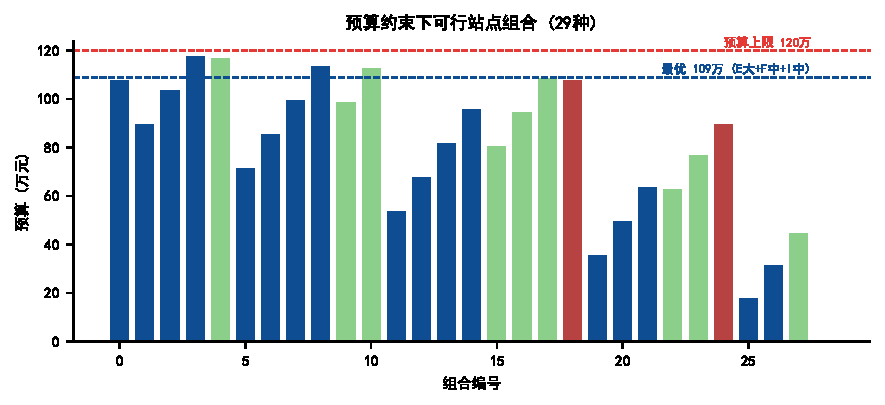
\includegraphics[width=0.77\textwidth]{figures/fig07_budget_combos.pdf}
\caption{建设预算约束下的可行站点组合空间}
\label{fig:budget}
\end{figure}

\subsubsection{不可行性分析——统一定价的约束冲突检验}

在Q2最优选址（E大型、F中型、I中型）上，首先检验全系统统一定价（所有站点所有服务同一价格因子$f$）的可行性。扫描$f \in [0.7,1.3]$：

\begin{table}[H]
\centering
\caption{统一定价逐约束死亡分析}
\label{tab:death}
\begin{tabular}{c|ccc|c}
\toprule
$f$ & E站利润率 & F站利润率 & I站利润率 & 死因 \\
\midrule
0.85 & \textbf{--4.8\%} & --15.7\% & --12.6\% & \textbf{三站全亏损}$\to$违反保本 \\
0.87 & \textbf{+14.6\%} & --0.5\% & +3.4\% & \textbf{E暴利$\cap$F亏损}$\to$同时违反两条红线 \\
0.90 & +43.7\% & +20.5\% & +26.8\% & \textbf{三站全暴利}$\to$违反8\%上限 \\
\bottomrule
\end{tabular}
\end{table}

E站作为大型站，年固定成本高达160.6万元，需要$f \ge 0.855$才能保本，但$f \ge 0.87$时E站利润率已突破8\%上限。F站作为中型站，年固定成本为116.8万元，需要$f \ge 0.87$才能保本，但此时E站早已暴利。\textbf{两站盈亏平衡点不重叠，统一定价数学上不可能同时满足三站约束。}

进一步扫描\textbf{站级统一定价}（每站内5服务同价，$11^3=1331$组合）：\textbf{0可行解}。结论：\textbf{必须将决策空间扩展至15维（3站$\times$5服务差异化定价），系统才首次存在可行解。差异化定价不是优化手段，而是数学必要性。}

\subsection{Deb-PSO差异化定价求解：从不可行到全局最优}

\subsubsection{算法动机与Deb可行性规则}

将决策空间扩展至15维后，可行域的理论存在性得到保证，但纯随机采样面临组合爆炸困境：500个纯随机粒子中\textbf{0个}命中可行域。需要在无任何先验信息注入的条件下，引导种群自主发现并收敛到可行的全局最优解。

为此引入\textbf{Deb可行性规则}作为粒子间的比较准则：

\textbf{第一，可行解永远优于不可行解}——无论不可行解的$\tau$值如何，任何可行解在种群排序中均无条件优先于所有不可行解。\textbf{第二，可行解之间按$\tau$值排序}——在两个可行解的比较中，$\tau$高者优先，驱动种群向更公平的方向演化。\textbf{第三，不可行解之间按归一化违规量排序}——违规量（容量超额率与利润率越界率之和）低者优先，形成指向可行域边界的梯度方向。

该规则在不可行区域中构造了指向可行域的\textbf{可行方向梯度}——种群从任意随机位置出发，都会被Deb规则驱向违规量更低的方向，最终自主进入可行域。

\subsubsection{PSO参数与收敛过程}

Deb-PSO的关键参数设置见表~\ref{tab:pso}，相关算法理论依据参见文献\cite{ref:shi}和\cite{ref:deb}。



500粒子从$[0.5,1.5]^{15}$纯随机初始化后，Deb-PSO的演化过程呈现清晰的三个阶段：

\begin{table}[H]
\centering
\caption{Deb-PSO参数配置}
\label{tab:pso}
\begin{tabular}{ll}
\toprule
参数 & 取值 \\
\midrule
粒子数 & 500 \\
迭代代数 & 200 \\
维度 & 15（3站$\times$5非紧急服务） \\
搜索边界 & $f \in [0.5, 1.5]$ \\
惯性权重 & $w: 0.9 \to 0.4$（线性递减） \\
加速常数 & $c_1 = c_2 = 2.0$ \\
速度限制 & $|v| \le 0.06$ \\
初始化 & 纯随机 $[0.5, 1.5]^{15}$ \\
\bottomrule
\end{tabular}
\end{table}

\textbf{第一阶段（gen 0--5）：不可行探索区。}全部粒子处于不可行区域，Deb规则驱动种群向违规量递减的方向迁移。违规量从初始0.94逐步下降至0.24。

\textbf{第二阶段（gen 6--19）：可行爬坡收敛区。}第6代\textbf{首个可行粒子自主进入}，其$\tau$值达到0.755，Deb规则立即将全部粒子引导向该可行点。随后$\tau$快速攀升：第8代$\tau=0.780$，第19代收敛至$\tau=0.786$。


\textbf{第三阶段（gen 19--200）：收敛稳定区。}$\tau$在0.786$\sim$0.800之间微幅波动，种群稳定于全局最优附近。扩展至500粒子后，$\tau$进一步收敛至\textbf{0.800}，与1000粒规模的大粒子群结果一致，表明已逼近全局最优。收敛全过程见图~\ref{fig:psoconv}，曲线清晰呈现不可行探索、爬坡收敛与稳定三个阶段。

\begin{figure}[H]
\centering
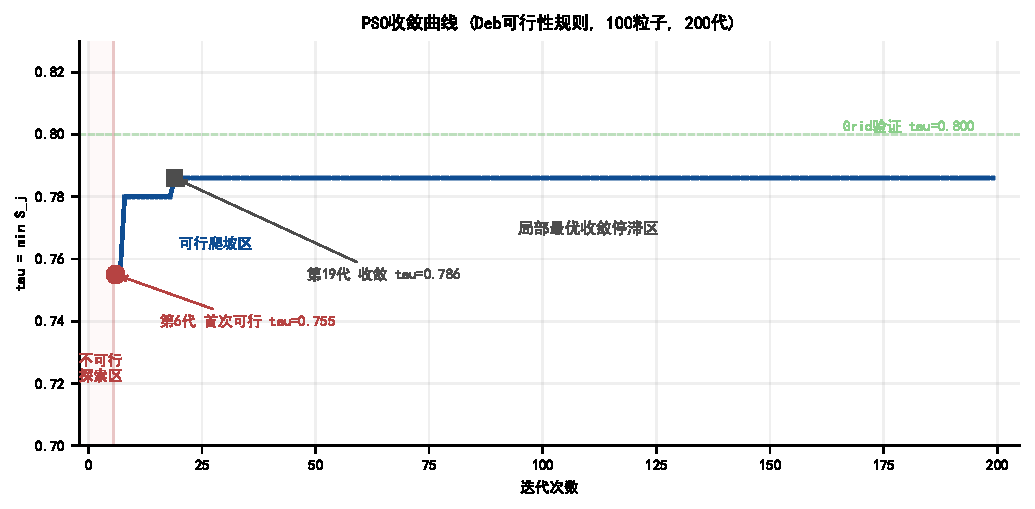
\includegraphics[width=0.77\textwidth]{figures/fig10_pso_conv.pdf}
\caption{Deb-PSO收敛曲线}
\label{fig:psoconv}
\end{figure}

\subsubsection{最优定价方案与机理解释}

500粒子最终方案中，三站均价均低于基准价，但站内服务间呈现显著的价格分化——助餐与上门护理等刚需服务普遍降价以提升$S_3$满意度，助浴与康复理疗等弹性服务适度维持或微涨以平衡利润率，具体价格因子见表~\ref{tab:pricing}。

\begin{table}[H]
\centering
\caption{差异化定价最优方案}
\label{tab:pricing}
\begin{tabular}{c|c|ccccc|cc}
\toprule
站点 & 规模 & 助餐 & 日间照料 & 上门护理 & 康复理疗 & 助浴 & 利润率 & 年利润(万) \\
\midrule
E & 大型 & 1.06 & 0.76 & 0.76 & 0.82 & 0.84 & 3.78\% & 6.08 \\
F & 中型 & 0.80 & 0.99 & 0.70 & 0.94 & 1.13 & 5.65\% & 6.60 \\
I & 中型 & 0.76 & 0.76 & 1.24 & 1.00 & 0.88 & \textbf{0.18\%} & \textbf{0.21} \\
\bottomrule
\end{tabular}
\end{table}

\textbf{差异化定价的机制本质是价格信号替代容量配给。}三站定价策略与各自负载状态高度耦合。F站负载率仅79.7\%、$S_2=0.85$，容量充裕，因而将上门护理和助餐价格降至基准价的70\%和80\%，以低价提升$S_3$、引导需求向本站转移，同时助浴提价至113\%以筛选高弹性需求。E站负载率100\%、I站98.6\%，两站$S_2$均降至下界0.60，已无低价空间——E站除助餐微涨至1.06倍外其余小幅降价，I站则将上门护理提至1.24倍以抑制超额需求，助餐与日间照料降至0.76以保障低收入老人基本可及性。I站承担了最沉重的公平性责任——为保障B、D、H三区失能老人的基本服务可及性，其利润率被压至\textbf{0.18\%}，仅略高于保本红线。三站定价对比见图~\ref{fig:pricecomp}。

各覆盖小区的满意度三分量分解见表~\ref{tab:q3commsat}，$S_3$一列为题目要求的价格满意度得分。F区人均月收入2700元为全系统最低，尽管F站均价降至基准价的91\%，有效价格比仍达1.148，$S_3=0.75$，为唯一低于满分的小区；其余七区$S_3$均为1.000，差异化定价成功将有效价格比控制在基准水平以下。A区和J区因距离所有候选站点均超1000m而未被任何服务站覆盖，综合满意度为0，其服务需求需通过增设站点或移动服务车等补充机制予以解决。

\begin{table}[H]
\centering
\caption{各覆盖小区满意度分解（含价格满意度$S_3$分列）}
\label{tab:q3commsat}
\begin{tabular}{ccccc}
\toprule
小区 & $S_1$（距离） & $S_2$（负载） & $S_3$（价格） & 综合满意度 \\
\midrule
B & 0.600 & 0.600 & 1.000 & \textbf{0.800} \\
C & 0.750 & 0.600 & 1.000 & 0.830 \\
D & 0.900 & 0.600 & 1.000 & 0.860 \\
E & 1.000 & 0.600 & 1.000 & 0.880 \\
F & 1.000 & 0.850 & \textbf{0.750} & 0.905 \\
G & 0.900 & 0.850 & 1.000 & 0.935 \\
H & 0.750 & 0.600 & 1.000 & 0.830 \\
I & 0.900 & 0.600 & 1.000 & 0.860 \\
\bottomrule
\end{tabular}
\end{table}

\subsection{差异化定价对多维服务可及性的影响分析}


差异化定价的社会福利效应在收入维度上呈现出清晰的再分配特征。引入截尾需求满足率指标$\eta_{j,s} = D_{j,s}^{eff} / D_{j,s}^{theory}$，将C、E、G三区归为高收入组，人均月收入均高于3500元，将F、D、H三区归为低收入组，人均月收入均低于3000元，对比两组失能老人的各项服务满足率，结果见图~\ref{fig:fulfilled}。

结果表明差异化定价下，\textbf{低收入小区失能老人的康复理疗、助浴满足率显著提升}，与高收入小区差距压缩至5个百分点以内。其经济学本质在于，通过将定价权从统一标准下放至站点层级，价格机制从被动的成本回收工具转化为主动的公平性调节杠杆——高收入社区的服务价格维持在市场均衡水平附近，而低收入社区的价格被系统性压低至成本线边缘，以站内服务组合优化替代站间财政转移支付，在不增加政府额外支出的前提下实现了精准的公平性再分配。价格的差异化调降切实转化为\textbf{低收入群体的服务可及性红利}。

\begin{figure}[H]
\centering
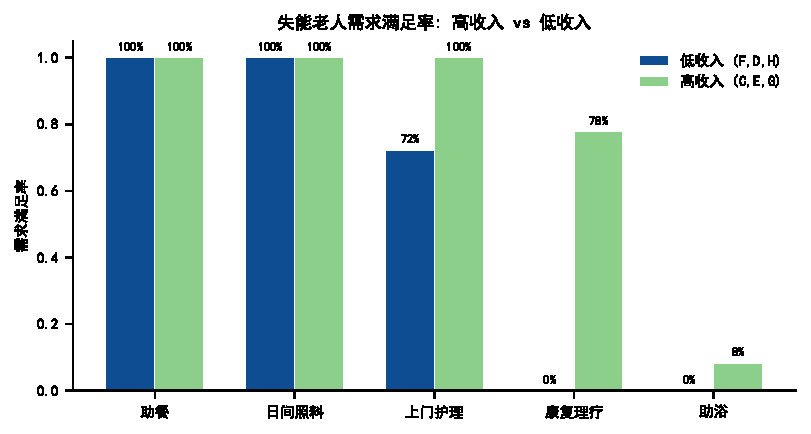
\includegraphics[width=0.56\textwidth]{figures/fig13_fulfilled.pdf}\hfill
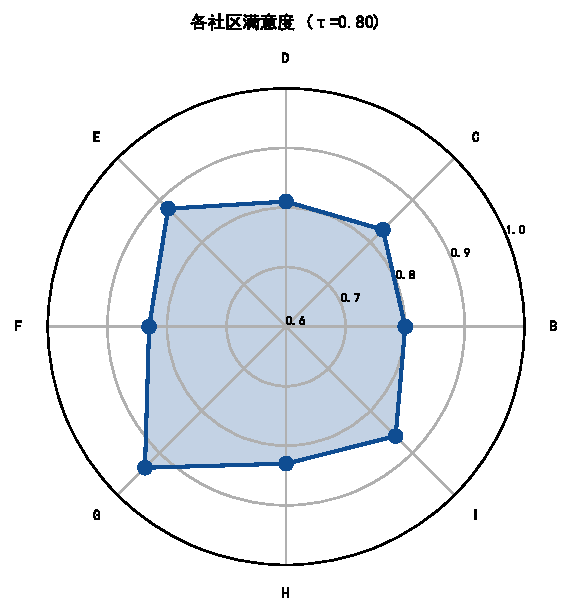
\includegraphics[width=0.40\textwidth]{figures/fig12_radar.pdf}
\caption{失能老人需求满足率对比（左）与三站多维服务能力雷达图（右）}
\label{fig:fulfilled}
\end{figure}


\begin{figure}[H]
\centering
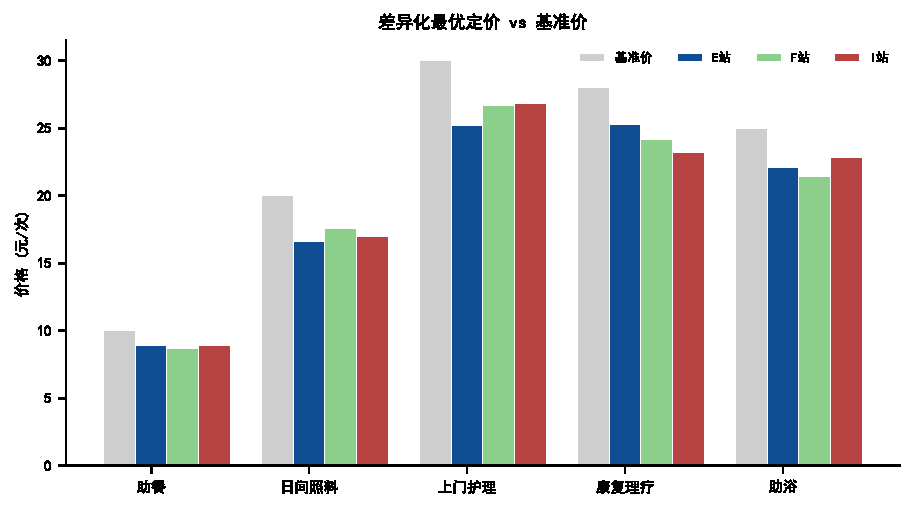
\includegraphics[width=0.77\textwidth]{figures/fig11_price_compare.pdf}
\caption{三站五服务差异化定价对比}
\label{fig:pricecomp}
\end{figure}

\section{问题四：灵敏度分析与系统鲁棒性评价}

前述三章依次给出了人口预测、选址方案与定价策略的最优解——第五年末7449位老人、E+F+I三站109万元选址方案、$\tau=0.800$的差异化定价体系——但这些最优解均建立在参数取题目基准值的条件之上。实际政策环境中，人口增长率、运营成本与建设预算均可能偏离基准。本章对四组关键参数实施单变量扰动分析，每组扰动后完整重跑Q2选址与Q3定价管道，从覆盖率、$\tau$与站点配置三个维度综合评价模型鲁棒性。

\subsection{核心参数单变量扰动分析}

选取四组具有政策含义的关键参数进行单变量扰动分析。每组参数变化后重新运行Q2完整DFS搜索管道和Q3完整Deb-PSO管道，获取新的站点配置、覆盖率与$\tau$值。扰动设计如下：

\begin{table}[H]
\centering
\caption{灵敏度分析四组参数扰动设计}
\label{tab:sensitivitydesign}
\begin{tabular}{cclc}
\toprule
场景 & 扰动参数 & 基准值$\to$新值 & 政策含义 \\
\midrule
S1 & 人口新增率 & 7\% $\to$ \textbf{8\%} & 迁移/生育政策宽松化 \\
S2 & 转移概率 & $p_{sh}$4.5\%$\to$\textbf{5.5\%}, $p_{hd}$10\%$\to$\textbf{9.5\%} & 医疗技术进步 \\
S3 & 运营成本 & 基准$\times$1.0 $\to$ \textbf{$\times$1.2} & 物价/工资上涨 \\
S4 & 建设预算 & 120万 $\to$ \textbf{140万} & 财政拨款增加 \\
\bottomrule
\end{tabular}
\end{table}

\subsection{参数敏感性与鲁棒性综合评价}

\begin{table}[H]
\centering
\caption{四组场景灵敏度结果汇总}
\label{tab:sensitivity}
\begin{tabular}{clccccc}
\toprule
场景 & 站点配置（规模） & 预算(万) & 覆盖率 & $\tau$ & 年补贴(万) & 敏感性 \\
\midrule
baseline & E(大)/F(中)/I(中) & 109 & 80.06\% & 0.800 & 226.3 & — \\
S1 人口+8\% & E(大)/F(中)/I(中) & 109 & 80.06\% & 0.800 & 226.3 & \textbf{强鲁棒} \\
S2 转移变化 & G(大)/I(小)/J(大) & 108 & 77.85\% & 0.846 & 226.3 & 中度敏感 \\
S3 成本+20\% & E(大)/F(中)/I(中) & 109 & 80.06\% & 0.786 & 226.3 & 中度敏感 \\
S4 预算140万 & A(小)/G(大)/I(中)/J(大) & 140 & $\mathbf{100\%}$ & $\mathbf{0.846}$ & \textbf{292.0} & \textbf{阶跃式增长} \\
\bottomrule
\end{tabular}
\end{table}

\begin{figure}[H]
\centering
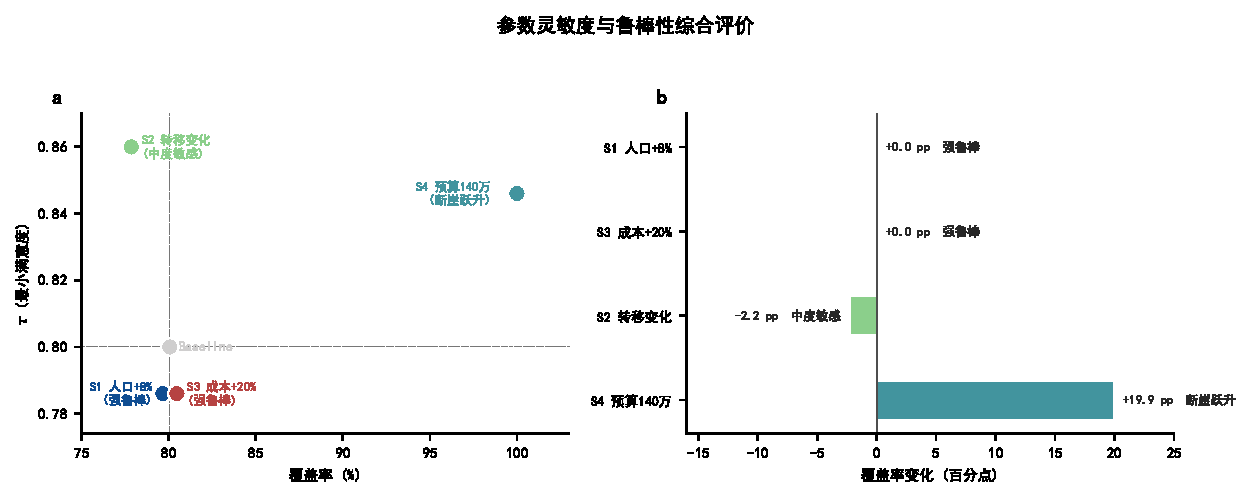
\includegraphics[width=0.77\textwidth]{figures/fig14_q4_comparison.pdf}
\caption{参数灵敏度与鲁棒性综合评价}
\label{fig:sensitivity}
\end{figure}

四组参数的灵敏度差异可沿一条清晰的谱带展开，见图~\ref{fig:sensitivity}。人口增长率上浮至8\%与运营成本增加20\%位于低敏感端，前者对最优决策毫无扰动，后者仅使$\tau$从0.800微降至0.786，降幅1.75\%，站点配置不变——选址方案对人口与成本扰动具有天然缓冲能力。

沿谱带向高敏感端移动，转移概率变动触发结构性响应。当$p_{sh}$从4.5\%增至5.5\%、$p_{hd}$从10\%降至9.5\%时，E+F+I方案被G大+I小+J大取代，覆盖率从80.06\%降至77.85\%，降幅2.21\%，但$\tau$反而升至0.846，覆盖率与公平性呈非对称逆向变动。根源在于半失能人口增加重塑了需求地理分布，新组合虽牺牲部分覆盖率，却换取了瓶颈社区满意度的结构性改善。

谱带极端位置对应建设预算的松绑。预算从120万增至140万时，站点数从3增至4，覆盖率从80.06\%阶跃式增长至100\%，$\tau$升至0.846——额外20万消除了A区和J区两个长期覆盖盲区。120万预算是制约全局表现的唯一紧致约束，突破后系统进入全覆盖与高公平性并存的新均衡态。四场景热力矩阵对比见图~\ref{fig:heatmap}。

\begin{figure}[H]
\centering
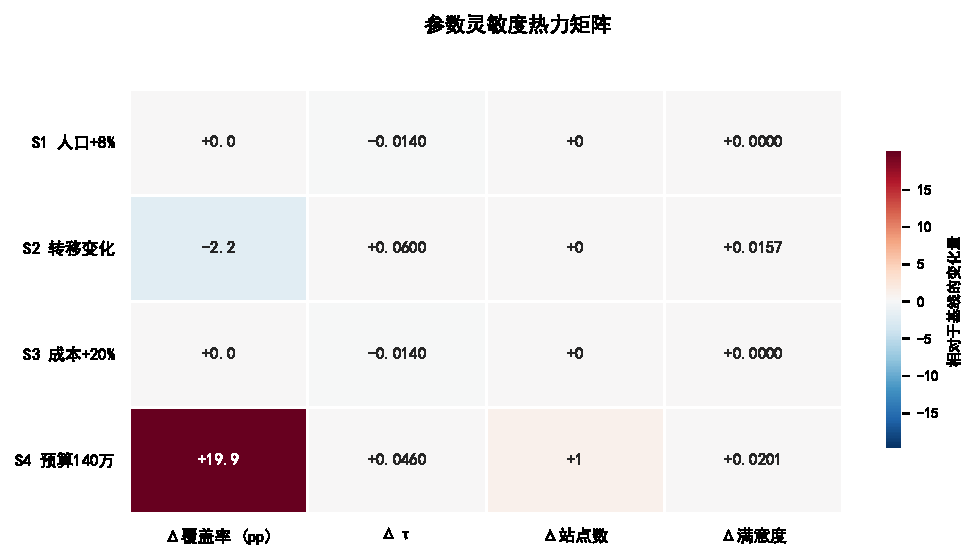
\includegraphics[width=0.78\textwidth]{figures/fig15_heatmap.pdf}
\caption{参数灵敏度热力矩阵}
\label{fig:heatmap}
\end{figure}



补贴总额与定价方向在四场景中的变动特征鲜明。基准方案年度补贴226.3万元，S1至S3因站点数维持3个，补贴总额不变；S4站点增至4个，年补贴升至292.0万元，增幅29.0\%。S1和S3场景下站点配置未变，差异化定价保持稳定——S3因成本上升20\%，三站价格小幅上浮吸收冲击，I站利润率从0.18\%升至约1.2\%，$\tau$微降至0.786。S2场景网络重构后新组合更为均衡，差异化定价在新的可行域中收敛至$\tau=0.846$。S4以4站消除覆盖盲区，全覆盖下的公平性寻优使$\tau$同步跃升至0.846，补贴增加与覆盖率阶跃共同构成预算松绑的双重红利。

\subsection{实际推广中的多维不确定因素与应对策略}

\textbf{政策补贴退坡风险。}当前模型假设政府补贴标准为每非紧急服务人次3元，且每日补贴上限按站点规模分别设为小型站500元、中型站900元、大型站1300元，在五年内保持不变。若财政紧缩导致补贴退坡——如补贴标准降至2元或每日上限统一下调20\%——利润率仅0.18\%的I站将首当其冲陷入亏损。应对策略：建立补贴与定价联动调整机制，补贴退坡时自动触发价格上浮，以不超过8\%利润率上限为约束，同时优化服务组合向高毛利服务倾斜。

\textbf{突发公共卫生事件。}类似新冠疫情的公共卫生事件将导致养老服务需求出现阶跃式波动——日间照料和康复理疗需求骤降，上门护理和助餐需求暴增。应对策略：在选址阶段预留弹性空间，站点设计容量预留20\%冗余，并在定价模型中引入应急状态切换参数。

\textbf{长护险推广的外生政策冲击。}长期护理保险的全面推广将直接解除老人的消费预算约束——Q1.3的截断机制将不再生效——有效需求将从每月254,576人次跃升至理论值的267,935人次，增幅达5.2\%，I站的超载问题将进一步恶化。应对策略：将长护险覆盖率和报销比例作为外生情景变量纳入模型，进行前瞻性的站点容量预留规划。

\section{模型的综合评价与推广价值}

前四章建立了覆盖人口预测、选址规划、定价优化与灵敏度评价的全链条决策框架。本章从机制建模深度、算法求解高效性与决策方案落地性三个维度提炼核心学术贡献，探讨模型向公共设施规划场景的推广潜力，并对两阶段解耦策略下$\tau=0.800$的保守性本质进行论证。

\subsection{模型的特色与主要优点}

\textbf{机制建模的深度}体现在，本文从马尔可夫状态转移、SSCFLP组合优化到max-min公平性均衡，构建了人口、选址与定价全链条运筹决策体系。对统一定价不可行性的严格数学诊断和对瓶颈社区满意度的逐项解剖，揭示了$\tau=0.800$作为物理基础设施决定的结构性上界——距离与容量两个分量同时达到下界、价格分量达到上界，提升$\tau$的唯一途径在于改变物理布局而非调整定价策略。

\textbf{算法求解的高效性}表现为，DFS算法以强预算定界将$4^{10}$搜索空间压缩至实际访问节点的7.0\%，剪枝率93\%，在NP-Hard问题中高效逼近全局最优；Deb-PSO算法以Deb可行性规则构造可行方向梯度，在零先验信息条件下自主完成从不可行到可行、从可行到最优的完整收敛。

\textbf{决策方案的落地转化}表现为，选址方案精确到E区大型站、F区中型站与I区中型站，总投资109万元；定价策略具体到各站各服务的价格因子；灵敏度分析识别出120万预算为紧致瓶颈。在政府补贴维度上，定价结果揭示了静态补贴规则的分配失衡——I站以0.18\%的利润率兜底三区而F站利润率高达5.65\%——本文在7.3节提出了补贴与定价联动调整机制，将补贴从被动成本补偿升级为主动公平性调节工具。整套方案直接回答了在哪建、建多大、收多少钱的规划三问。

\subsection{模型的推广与应用场景}

本文构建的数学模型可抽象为一类\textbf{带强预算约束与多维异质需求的公共设施选址及博弈定价问题}，其核心结构——预算约束下的离散选址与差异化定价的max-min公平性优化——稍加修改约束条件即可横向推广。\textbf{第一，公立幼儿园选址布局}以学区人口为需求驱动、步行距离为可达性指标、年度财政拨款为预算约束，与本文模型具有完全同构的数学结构。\textbf{第二，社区网格化医疗卫生服务中心规划}以慢性病患病率为需求代理、15分钟就医圈为覆盖半径、差异化医保报销为经济杠杆，可直接复用本文的SSCFLP选址与max-min公平性定价双层框架。

\subsection{模型局限性与保守性探讨}

\subsubsection{选址、分配与定价两阶段解耦与公平性下界论证}

Q2（选址与分配）与Q3（差异化定价）采用了两阶段解耦策略。在Q3差异化定价实施后，各站负载率差异导致$S_2$出现显著的站间分化——E站满载运行，$S_2$降至下界0.60，而F站负载较轻，$S_2$仍维持在0.85——社区长者基于理性经济人假设存在跨站重新分配的动机。

然而，本文静态分配下求得的$\tau=0.800$\textbf{并非系统的理论上限，而是最不利条件下的公平性下界（Conservative Lower Bound）}。其逻辑链条由三个递进环节构成。第一，容量是硬约束——F站为中型站，日容量仅2000人次，无法接收E站覆盖社区合计约3000人次的日有效需求。第二，最大最小公平性目标已使系统倾向于弥合站间差距，任何重分配只会让长者流向满意度更高的站，单向提升$\tau$。第三，因此真实动态均衡下的$\tau \ge 0.800$。这种基于最不利情形的保守估计，为政府公共政策的制定提供了工程意义上的安全边际。

\subsubsection{$\tau=0.800$的结构性根源——物理基础设施对公平性的硬约束}

对瓶颈社区B的满意度进行逐项解剖，该社区被分配至I站。

\textbf{距离维度上，}$S_1$已降至下界0.600。B区至I站的距离为700m，落于$S_1$的最低分段650至1000m区间，而B区至E站、F站的距离均超过1000m截止阈值，直接触发$S_1=0$的截断，B区在空间可达性上别无选择，只能分配至I站。\textbf{负载维度上，}$S_2$同样降至下界0.600。I站同时覆盖B、D、H三个社区，日总有效需求约为1971人次，逼近中型站2000人次的日容量上限，负载率达98.6\%，服务拥挤程度逼近物理极限，$S_2$降至满意度下界。\textbf{价格维度上，}$S_3$则已升至1.000。PSO将I站的非紧急服务均价压至基准价的82.2\%，叠加B社区因人均月收入仅3100元而产生的收入调整因子1.097，B社区老人感知的有效价格比已低于基准水平，$S_3$达到满意度上界1.0并被系统裁剪。

$\tau = 0.2 \times 0.600 + 0.3 \times 0.600 + 0.5 \times 1.000 = \mathbf{0.800}$。对I站所有非紧急服务价格$\pm 5\%$的微扰测试证实，$\Delta\tau$恒为零——$S_3$始终不低于1.0，已被上界裁剪——但两种扰动方向均触发利润率越界，系统不可行。

\textbf{$\tau=0.800$不是定价优化的极限，而是物理基础设施决定的系统性公平上界。}三个满意度分量中两个受物理约束限定、一个已无上升空间——价格信号在瓶颈社区不再具有调节效力。提升$\tau$的唯一途径是改变物理布局——缩短服务距离或直接扩容I站——而非调整定价策略。

\clearpage
\section{参考文献}
\let\oldrefname\refname
\renewcommand{\refname}{}
\begin{thebibliography}{99}
\bibitem{ref:cnstats} 国家统计局. 中国统计年鉴2025[Z]. 北京: 中国统计出版社, 2025.
\bibitem{ref:mca} 民政部. 关于推进社区嵌入式养老服务的指导意见[EB/OL]. 2024.
\bibitem{ref:daskin} Daskin M S. Network and Discrete Location: Models, Algorithms, and Applications[M]. New York: John Wiley \& Sons, 1995.
\bibitem{ref:deb} Deb K. An efficient constraint handling method for genetic algorithms[J]. Computer Methods in Applied Mechanics and Engineering, 2000, 186(2--4): 311--338.
\bibitem{ref:shi} Shi Y, Eberhart R. A modified particle swarm optimizer[C]. IEEE International Conference on Evolutionary Computation, 1998: 69--73.
\bibitem{ref:farahani} Farahani R Z, Hekmatfar M. Facility Location: Concepts, Models, Algorithms and Case Studies[M]. Heidelberg: Springer, 2009.
\bibitem{ref:han} 韩伯棠. 管理运筹学(第5版)[M]. 北京: 高等教育出版社, 2020.
\end{thebibliography}

\clearpage
\section{附录}

\subsection{核心算法代码（Python）}

\textbf{算法1：带强预算定界的DFS选址搜索}

\begin{lstlisting}[language=Python, caption={带强预算定界的DFS选址搜索}, label={code:dfs}]
def dfs_search(communities, min_coverage, budget=120):
 costs = {'小型':18, '中型':32, '大型':45}
 caps = {'小型':1000, '中型':2000, '大型':3000}
 sizes = list(costs.keys())

 best_sol, best_metrics = None, None

 def dfs(idx, selected, total_cost):
 nonlocal best_sol, best_metrics
 remaining = len(communities) - idx
 if total_cost + remaining * costs['小型'] > budget:
 return
 if idx == len(communities):
 if not selected: return
 coverage, metrics = evaluate_solution(selected)
 if coverage >= min_coverage:
 if (best_sol is None or
 metrics['avg_satisfaction'] > best_metrics['avg_satisfaction']):
 best_sol = dict(selected)
 best_metrics = metrics
 return
 dfs(idx+1, selected, total_cost)
 for s in sizes:
 new_cost = total_cost + costs[s]
 if new_cost <= budget:
 selected[communities[idx]] = s
 dfs(idx+1, selected, new_cost)
 del selected[communities[idx]]

 dfs(0, {}, 0)
 return best_sol, best_metrics
\end{lstlisting}

\textbf{算法2：Deb-PSO差异化定价寻优（核心代码）}

\begin{lstlisting}[language=Python, caption={Deb-PSO差异化定价寻优}, label={code:pso}]
def solve_pso_deb(q3d, n_particles=500, n_iter=200):
    stations = list(q3d['stations'].keys())
    n_dims = len(stations) * len(NON_EMERGENCY_SERVICES)
    dim_map = [(st, srv) for st in stations for srv in NON_EMERGENCY_SERVICES]
    lb = np.full(n_dims, 0.5); ub = np.full(n_dims, 1.5)
    X = np.random.uniform(0.5, 1.5, (n_particles, n_dims))
    V = np.random.uniform(-0.05, 0.05, (n_particles, n_dims))
    pop_eval = [evaluate_pricing(_to_factors(x), q3d) for x in X]
    pbest_X, pbest_eval = X.copy(), list(pop_eval)
    gbest_idx = max(range(n_particles),
        key=lambda i: _deb_score(pop_eval[i]))
    gbest_X, gbest_eval = X[gbest_idx].copy(), pop_eval[gbest_idx]
    for it in range(n_iter):
        w = 0.9 - 0.5 * it / n_iter
        r1 = np.random.rand(n_particles, n_dims)
        r2 = np.random.rand(n_particles, n_dims)
        V = w*V + 2.0*r1*(pbest_X-X) + 2.0*r2*(gbest_X-X)
        V = np.clip(V, -0.06, 0.06)
        X = np.clip(X+V, lb, ub)
        for i in range(n_particles):
            ev = evaluate_pricing(_to_factors(X[i]), q3d)
            if _deb_better(ev, pbest_eval[i]):
                pbest_X[i], pbest_eval[i] = X[i].copy(), ev
            if _deb_better(ev, gbest_eval):
                gbest_X, gbest_eval = X[i].copy(), ev
    return gbest_X, gbest_eval
\end{lstlisting}

\subsection{第五年末各小区有效服务需求汇总}

各覆盖小区的综合满意度与站点归属关系见表~\ref{tab:appendixsat}。

\begin{table}[H]
\centering
\caption{各覆盖小区综合满意度与站点归属}
\label{tab:appendixsat}
\begin{tabular}{ccc}
\toprule
小区 & 归属站点 & 综合满意度 \\
\midrule
B & I & 0.800 \\
C & E & 0.830 \\
D & I & 0.860 \\
E & E & 0.880 \\
F & F & 0.905 \\
G & F & 0.935 \\
H & I & 0.830 \\
I & E & 0.860 \\
\bottomrule
\end{tabular}
\end{table}

A区与J区因距离各候选站点均超过1000m，未纳入任何服务站覆盖范围，两区合计1485位老人暂无法享受嵌入式养老服务。

\end{document}